% -*-LaTeX-*-

%%  Copyright (C) 2011 Vincent Rahli
%%  Permission is granted to copy, distribute and/or modify this document
%%  under the terms of the GNU Free Documentation License, Version 1.3
%%  or any later version published by the Free Software Foundation;
%%  with no Invariant Sections, no Front-Cover Texts, and no Back-Cover Texts.
%%  A copy of the license is included in the section entitled "GNU
%%  Free Documentation License".


\documentclass[final]{article}
%\documentclass[draft]{article}


%%%% PACKAGES

\usepackage{amsmath}
\usepackage{url}
\usepackage{float}
\usepackage{proof}
\usepackage{color}
\usepackage{graphicx}
\usepackage{listings}
\usepackage[nomargin,inline]{fixme}
\usepackage{changepage}
\usepackage{{../../tex/bsymb}}
\usepackage{{../../tex/stmaryrd}}
\usepackage{{../../tex/nuprl}}


%%%% LISTING

% -*-LaTeX-*-


\RequirePackage{listings}
\RequirePackage{color}

\definecolor{EMLgreen}{cmyk}{0.7,0.1,0.7,0.3}
\definecolor{EMLpurple}{cmyk}{0,0.56,0.14,0.29}
\definecolor{EMLpeach}{cmyk}{0,0.4,0.8,0.2}
\definecolor{EMLred}{cmyk}{0,1,1,0.1}
%\definecolor{EMLblue}{cmyk}{0.31,0.18,0.0,0.41}
\definecolor{EMLblue}{cmyk}{0.48,0.20,0.0,0.50}

\lstdefinelanguage
    {EventML}
    {
      basicstyle=\sffamily,
      %basicstyle=\small\sffamily,
      %basicstyle=\small\bfseries,
      %basicstyle=\small\ttfamily,
      morekeywords=[1]{or,if,then,else,let,letrec,in,match,of,infix,infixr,%
        parameter,constant,import,export,input,output,internal,base,send,%
        main,type,Prior,self,specification,broadcast,Once,where,with,%
        case,op,class,classrec,until,OnLoc,Skip,invariant,progress,ordering,%
        on,variable,Output,forall,exists,locations,parameters,messages,o,O,%
        consistency,memory,and,options,abstype,assume,observes,guarantee,%
        State,Memory},
      keywordstyle=[1]\color{EMLpurple},
      morekeywords=[2]{Bag,Loc,List,Int,Bag,Bool,Unit,Deq,Type,Prop,Event,Tok},
      keywordstyle=[2]\color{EMLgreen},
      morekeywords=[3]{fst,snd,inl,inr,isl,fix,not,before,location},
      keywordstyle=[3]\color{EMLblue},
      alsoletter={'},
      sensitive,%
      morecomment=[n]{(*}{*)},
      commentstyle=\color{EMLred},
      morestring=[b]",
      moredelim=[s][\color{EMLpeach}]{``}{``},
      %morecomment=[n]{`}{`},
      literate=*{/}{$/$}1 {-}{$\mbox{-}$}1, %{->}{$\rightarrow$ }2,% {=>}{$\Rightarrow$ }2,
      %=\color{lightgray},
      %backgroundcolor=\color{lightgray},
      %moredirectives={open,close,include}%
    }

\lstset{basicstyle=\small,language=EventML}


%%%% FIXME

\fxusetheme{color}
\fxuseenvlayout{color}


%%%% BIBLIOGRAPHY

\bibliographystyle{alpha}


%%%% MACROS

\newcommand{\SET}[1]{\mathsf{#1}}

\newcommand{\SETtoset}[1]{\pow(\SET{#1})}

\newcommand{\SETnat}[0]{\nat}
\newcommand{\SETvar}{\SET{Var}}
\newcommand{\SETexp}{\SET{Exp}}
\newcommand{\SETatexp}{\SET{AtExp}}
\newcommand{\SETpat}{\SET{Pat}}
\newcommand{\SETatpat}{\SET{AtPat}}
\newcommand{\SETint}{\SET{Int}}
\newcommand{\SETstring}{\SET{String}}
\newcommand{\SETatom}{\SET{Token}}
\newcommand{\SETcharseq}{\SET{CharSeq}}
\newcommand{\SETatoms}{\SET{Tokens}}
\newcommand{\SETatomsl}{\SET{TokensList}}
\newcommand{\SETatomsp}{\SET{PTokens}}
\newcommand{\SETop}{\SET{Op}}
\newcommand{\SETvid}{\SET{Vid}}
\newcommand{\SETbind}{\SET{Bind}}
\newcommand{\SETty}{\SET{Ty}}
\newcommand{\SETdec}{\SET{Dec}}
\newcommand{\SETldec}{\SET{LetDec}}
\newcommand{\SETcdec}{\SET{ClassDec}}
\newcommand{\SETtyvar}{\SET{TyVar}}
\newcommand{\SETeqtyvar}{\SET{EqTyVar}}
\newcommand{\SETtycon}{\SET{PTyC}}
\newcommand{\SETinftycon}{\SET{ITyC}}
\newcommand{\SETbool}{\SET{Bool}}
\newcommand{\SETparam}{\SET{Param}}
\newcommand{\SETityenv}{\SET{ITyEnv}}
\newcommand{\SETity}{\SET{ITy}}
\newcommand{\SETityseq}{\SET{ITySeq}}
\newcommand{\SETitypseq}{\SET{ITySeq}}
\newcommand{\SETityvar}{\SET{ITyVar}}
\newcommand{\SETityvarset}{\SET{ITyVarSet}}
\newcommand{\SETityscheme}{\SET{ITyScheme}}
\newcommand{\SETityfun}{\SET{ITyFun}}
\newcommand{\SETtypseq}{\SET{TySeq}}
\newcommand{\SETtypseqset}{\SET{TySeqSet}}
\newcommand{\SETtypvarseq}{\SET{TvSeq}}
\newcommand{\SETsub}{\SET{Sub}}
\newcommand{\SETprog}{\SET{Prog}}
\newcommand{\SETcrule}{\SET{CRule}}
\newcommand{\SETbrule}{\SET{BRule}}
\newcommand{\SETmrule}{\SET{MRule}}
\newcommand{\SETbagpat}{\SET{BagPat}}
\newcommand{\SETmsgpat}{\SET{MsgPat}}
\newcommand{\SETcasepat}{\SET{CasePat}}
\newcommand{\SETarg}{\SET{Arg}}
\newcommand{\SETargs}{\SET{Args}}
\newcommand{\SETbvars}{\SET{BVars}}
\newcommand{\SETheader}{\SET{Header}}
\newcommand{\SEThdrstatus}{\SET{Status}}
\newcommand{\SEThdropt}{\SET{HdrOpt}}
\newcommand{\SEThdropts}{\SET{HdrOpts}}
\newcommand{\SETnatnum}{\SET{Nat}}
\newcommand{\SETconst}{\SET{Const}}

\newcommand{\META}[1]{\mathit{#1}}

\newcommand{\METAtoset}[1]{\overline{\META{#1}}}
\newcommand{\METAtoseq}[1]{\overrightarrow{\META{#1}}}

\newcommand{\METAexp}{\META{exp}}
\newcommand{\METAvar}{\META{v}}
\newcommand{\METAatexp}{\META{atexp}}
\newcommand{\METApat}{\META{pat}}
\newcommand{\METAatpat}{\META{atpat}}
\newcommand{\METAint}{\META{i}}
\newcommand{\METAstring}{\META{s}}
\newcommand{\METAty}{\META{ty}}
\newcommand{\METAvid}{\META{vid}}
\newcommand{\METAop}{\META{op}}
\newcommand{\METAbind}{\META{bind}}
\newcommand{\METAdec}{\META{dec}}
\newcommand{\METAldec}{\META{ldec}}
\newcommand{\METAcdec}{\META{cdec}}
\newcommand{\METAtyvar}{\META{a}}
\newcommand{\METAtyvarset}{\METAtoset{\METAtyvar}}
\newcommand{\METAtyvarseq}{\METAtoseq{\METAtyvar}}
\newcommand{\METAeqtyvar}{\META{ea}}
\newcommand{\METAtycon}{\META{ptc}}
\newcommand{\METAinftycon}{\META{itc}}
\newcommand{\METAbool}{\META{b}}
\newcommand{\METAparam}{\META{p}}
\newcommand{\METAity}{\META{\tau}}
\newcommand{\METAityseq}{\METAtoseq{\METAity}}
\newcommand{\METAityset}{\METAtoset{\METAity}}
\newcommand{\METAityscheme}{\META{\sigma}}
\newcommand{\METAityschemeset}{\METAtoset{\sigma}}
\newcommand{\METAityfun}{\META{\delta}}
\newcommand{\METAityenv}{\META{\Gamma}}
\newcommand{\METAityvar}{\META{\alpha}}
\newcommand{\METAityvarset}{\METAtoset{\METAityvar}}
\newcommand{\METAityvarseq}{\METAtoseq{\METAityvar}}
\newcommand{\METAfun}{\META{f}}
\newcommand{\METAatom}{\META{tok}}
\newcommand{\METAcharseq}{\META{cseq}}
\newcommand{\METAatoms}{\META{toks}}
\newcommand{\METAatomsl}{\META{latoms}}
\newcommand{\METAatomsp}{\META{patoms}}
\newcommand{\METAtypseq}{\META{tyseq}}
\newcommand{\METAtypseqset}{\META{tyseqset}}
\newcommand{\METAtypvarseq}{\META{tvseq}}
\newcommand{\METAclass}{\META{C}}
\newcommand{\METAset}{\META{s}}
\newcommand{\METArel}{\META{rel}}
\newcommand{\METAtup}{\META{t}}
\newcommand{\METAsub}{\META{sub}}
\newcommand{\METAprog}{\META{prog}}
\newcommand{\METAcrule}{\META{crule}}
\newcommand{\METAbrule}{\META{brule}}
\newcommand{\METAmrule}{\META{mrule}}
\newcommand{\METAbagpat}{\META{bagpat}}
\newcommand{\METAmsgpat}{\META{msgpat}}
\newcommand{\METAcasepat}{\META{casepat}}
\newcommand{\METAarg}{\META{arg}}
\newcommand{\METAargs}{\META{args}}
\newcommand{\METAbvars}{\META{bvars}}
\newcommand{\METAheader}{\META{hdr}}
\newcommand{\METAeo}{\META{eo}}
\newcommand{\METAeclass}{\META{X}}
\newcommand{\METAevent}{\META{e}}
\newcommand{\METAhdrstatus}{\META{status}}
\newcommand{\METAhdropt}{\META{hdropt}}
\newcommand{\METAhdropts}{\META{hdropts}}
\newcommand{\METAnatnum}{\META{n}}
\newcommand{\METAconst}{\META{c}}

\newcommand{\MEM}[1]{\mathsf{#1}}

\newcommand{\MEMinfera}[1]{\infer[]{#1}{}}
\newcommand{\MEMinferb}[2]{\infer[]{#1}{#2}}
\newcommand{\MEMinferc}[3]{\infer[]{#1}{#2 & #3}}
\newcommand{\MEMinfercc}[3]{\infer[]{#1}{\begin{array}{l}#2 \\ #3\end{array}}}
\newcommand{\MEMinferd}[4]{\infer[]{#1}{#2 & #3 & #4}}
\newcommand{\MEMinferdd}[4]{\infer[]{#1}{\begin{array}{l}#2 \\ #3 \\ #4\end{array}}}
\newcommand{\MEMinferddd}[4]{\infer[]{#1}{\begin{array}{c@{\hspace{0.4in}}c}#2 & #3 \\ \multicolumn{2}{c}{#4}\end{array}}}
\newcommand{\MEMinfere}[5]{\infer[]{#1}{#2 & #3 & #4 & #5}}
\newcommand{\MEMinferee}[5]{\infer[]{#1}{\begin{array}{l}#2 \\ #3 \\ #4 \\ #5\end{array}}}
\newcommand{\MEMinferf}[6]{\infer[]{#1}{#2 & #3 & #4 & #5 & #6}}
\newcommand{\MEMinferff}[6]{\infer[]{#1}{\begin{array}{l}#2 \\ #3 \\ #4 \\ #5 \\ #6\end{array}}}
\newcommand{\MEMinferffp}[6]{\infer[]{#1}{\begin{array}{l}#2\ \ \ \ \ #3\ \ \ \ \ #4 \\ #5 \\ #6\end{array}}}
\newcommand{\MEMtyping}[3]{#1 : \mytuple{#2, #3}}
\newcommand{\MEMtypingexp}[3]{#1 : \mytuple{#2, #3}}
\newcommand{\MEMtypingpat}[3]{#1 :_{\mbox{p}} \mytuple{#2, #3}}
\newcommand{\MEMtypingseq}[3]{#1 :_{\mbox{s}} \mytuple{#2, #3}}
\newcommand{\MEMtypingtyseq}[2]{#1 :_{\mbox{s}} #2}
\newcommand{\MEMtypingty}[2]{#1 :_{\mbox{t}} #2}
\newcommand{\MEMtypingdec}[3]{#1 :_{\mbox{d}} \mytuple{#2, #3}}
\newcommand{\MEMtypinghdr}[3]{#1 :_{\mbox{h}} \mytuple{#2, #3}}
\newcommand{\MEMafunc}[2]{#1(#2)}
\newcommand{\MEMafuncat}[2]{#1[#2]}
\newcommand{\MEMfunc}[2]{#1\rightarrow#2}
\newcommand{\MEMinstance}[2]{#1 \prec #2}
\newcommand{\MEMtypeofopSYMB}{\MEM{typeOf}}
\newcommand{\MEMtypeofop}[1]{\MEMtypeofopSYMB(#1)}
\newcommand{\MEMrestrictoutSYMB}{\domsub}
\newcommand{\MEMrestrictout}[2]{#2\MEMrestrictoutSYMB#1}
\newcommand{\MEMdomSYMB}{\MEM{dom}}
\newcommand{\MEMdom}[1]{\MEMdomSYMB(#1)}
\newcommand{\MEMdisj}[1]{\MEM{dj}(#1)}
\newcommand{\MEMpowset}[1]{\pow(#1)}
\newcommand{\MEMpair}[2]{\llparenthesis#1,#2\rrparenthesis}
\newcommand{\MEMdunion}[2]{#1\uplus#2}
\newcommand{\MEMbrel}[3]{#1\ #2\ #3}
\newcommand{\MEMinverse}[1]{#1^{-1}}
\newcommand{\MEMranSYMB}{\MEM{ran}}
\newcommand{\MEMran}[1]{\MEMranSYMB(#1)}
\newcommand{\MEMrestrictinSYMB}[0]{\domres}
\newcommand{\MEMrestrictin}[2]{#2\MEMrestrictinSYMB#1}
\newcommand{\MEMuplusSYMB}{+}
\newcommand{\MEMuplus}[2]{#1\MEMuplusSYMB#2}
\newcommand{\MEMuplusop}[2]{#1\CONSop{\MEMuplusSYMB#2}}
\newcommand{\MEMplusenv}[2]{\MEMuplus{#1}{#2}}
\newcommand{\MEMplusopenv}[2]{\MEMuplusop{#1}{#2}}
\newcommand{\MEMequnionSYMB}[0]{\boxplus}
\newcommand{\MEMequnion}[2]{#1{\MEMequnionSYMB}#2}
\newcommand{\MEMuenvSYMB}[0]{\Cup}
\newcommand{\MEMuenv}[2]{#1\MEMuenvSYMB#2}
\newcommand{\MEMfintuple}[1]{\MEM{tuple}(#1)}
\newcommand{\MEMclosSYMB}{\MEM{clos}}
\newcommand{\MEMclos}[2]{\MEMclosSYMB_{#1}(#2)}
\newcommand{\MEMsub}[2]{#1[#2]}
\newcommand{\MEMfreetyvarsSYMB}{\MEM{fv}}
\newcommand{\MEMfreetyvars}[1]{\MEMfreetyvarsSYMB(#1)}
%\newcommand{\MEMinternalTySYMB}{\MEM{iTy}}
%\newcommand{\MEMinternalTy}[1]{\MEMinternalTySYMB(#1)}
%\newcommand{\MEMinternalTyseqSYMB}{\MEM{iTyseq}}
%\newcommand{\MEMinternalTyseq}[1]{\MEMinternalTyseqSYMB(#1)}
\newcommand{\MEMtoidSYMB}{\MEM{toid}}
\newcommand{\MEMtoid}[2]{\MEMtoidSYMB(#1,#2)}
\newcommand{\MEMtransSYMB}{\MEM{trans}}
\newcommand{\MEMtrans}[1]{\MEMtransSYMB(#1)}
\newcommand{\MEMoverloadSYMB}{\MEM{overload}}
\newcommand{\MEMoverload}[3]{\MEMoverloadSYMB(#1,#2,#3)}
\newcommand{\MEMadmitseqSYMB}{\MEM{admitsEq}}
\newcommand{\MEMadmitseq}[1]{\MEMadmitseqSYMB(#1)}
\newcommand{\MEMityenvop}{\MEM{\Gamma{op}}}
\newcommand{\MEMityenvlib}{\MEM{\Gamma{lib}}}

\newcommand{\CONS}[1]{\mathtt{#1}}
\newcommand{\CONSB}[1]{\textbf{\texttt{#1}}}

\newcommand{\CONSquot}{\textbf{\texttt{/}}\hspace{-0.05in}\sim}
\newcommand{\CONSunder}{\textbf{\texttt{\_}}}
\newcommand{\CONSpipe}{\textbf{\texttt{|}}}
\newcommand{\CONScomp}{\textbf{\texttt{o}}}
\newcommand{\CONSbcomp}{\textbf{\texttt{O}}}
\newcommand{\CONSlpar}{\textbf{\texttt{(}}}
\newcommand{\CONSrpar}{\textbf{\texttt{)}}}
\newcommand{\CONSsemicolon}{\textbf{\texttt{;}}}
\newcommand{\CONScolon}{\textbf{\texttt{:}}}
\newcommand{\CONSconslist}{\textbf{\texttt{.}}}
\newcommand{\CONSbinding}{\mathrel{\textbf{\texttt{>>}}}}
\newcommand{\CONSmonbindSYMB}{\textbf{\texttt{>>=}}}
\newcommand{\CONSmonbind}{\mathrel{\CONSmonbindSYMB}}
\newcommand{\CONSparallelSYMB}{\textbf{\texttt{||}}}
\newcommand{\CONSparallel}[2]{#1\ \CONSparallelSYMB\ #2}
\newcommand{\CONSdot}{\textbf{\texttt{.}}}
\newcommand{\CONSeq}{\textbf{\texttt{=}}}
\newcommand{\CONSat}{\textbf{\texttt{@}}}
\newcommand{\CONScomma}{\textbf{\texttt{,}}}
\newcommand{\CONSdarrow}{\textbf{\texttt{=>}}}
\newcommand{\CONSbackslash}{\textbf{\texttt{$\backslash$}}}
\newcommand{\CONSparen}[1]{\textbf{\texttt{(}}#1\textbf{\texttt{)}}}
\newcommand{\CONSpriorSYMB}{\CONS{Prior}}
\newcommand{\CONSprior}[1]{\CONSpriorSYMB(#1)}
\newcommand{\CONSonceSYMB}{\CONS{Once}}
\newcommand{\CONSonce}[1]{\CONSonceSYMB(#1)}
\newcommand{\CONSoutputSYMB}{\CONS{Output}}
\newcommand{\CONSoutput}[1]{\CONSoutputSYMB(#1)}
\newcommand{\CONSonlocSYMB}{\CONS{OnLoc}}
\newcommand{\CONSonloc}[1]{\CONSonlocSYMB(#1)}
\newcommand{\CONSinlSYMB}{\CONS{inl}}
\newcommand{\CONSinl}[1]{\CONSinlSYMB(#1)}
\newcommand{\CONSinrSYMB}{\CONS{inr}}
\newcommand{\CONSinr}[1]{\CONSinrSYMB(#1)}
\newcommand{\CONSbaseSYMB}{\CONS{Base}}
\newcommand{\CONSbase}[2]{\CONSbaseSYMB(#1\CONSat#2)}
\newcommand{\CONSbasehdropt}[1]{\CONS{base}\ #1}
\newcommand{\CONSsendhdropt}[1]{\CONS{send}\ #1}
\newcommand{\CONSbroadcasthdropt}[1]{\CONS{broadcast}\ #1}
\newcommand{\CONSmsgSYMB}{\CONS{MSG}}
\newcommand{\CONSmsg}[2]{\CONSmsgSYMB(#1,#2)}
\newcommand{\CONScaseexp}[2]{\CONS{case}\ #1\ #2}
\newcommand{\CONScasemsg}[2]{\CONS{caseMsg}\ #1\ #2}
\newcommand{\CONScasebag}[2]{\CONS{caseBag}\ #1\ #2}
\newcommand{\CONSmatchexp}[2]{\CONS{match}\ #1\ #2}
\newcommand{\CONScasen}[2]{\ \CONS{of}\ #1\ \cdots\ \CONS{of}\ #2}
\newcommand{\CONSmatchmsgn}[2]{\CONS{of}\ #1\ \cdots\ \CONS{of}\ #2}
\newcommand{\CONSmatchmsgna}[2]{\begin{array}[t]{l}\CONS{of}\ #1\\ \vdots\\ \CONS{of}\ #2\end{array}}
\newcommand{\CONSmrulemsg}[2]{#1\ \CONSdarrow\ #2}
\newcommand{\CONSmrulebag}[2]{#1\ \CONSdarrow\ #2}
\newcommand{\CONSmatchbagn}[2]{\CONS{of}\ #1\ \cdots\ \CONS{of}\ #2}
\newcommand{\CONSmatchn}[2]{\CONS{with}\ #1\ \cdots\ \CONS{with}\ #2}
\newcommand{\CONSmatchna}[2]{\begin{array}[t]{l}\CONS{with}\ #1\\ \vdots\\ \CONS{with}\ #2\end{array}}
\newcommand{\CONSmrule}[2]{#1\ \CONSdarrow\ #2}
\newcommand{\CONSopexp}[3]{#1\ #2\ #3}
\newcommand{\CONStypexp}[2]{#1 \CONScolon #2}
\newcommand{\CONStexp}[1]{\CONScolon\CONScolon#1}
\newcommand{\CONSappexp}[2]{#1\ #2}
\newcommand{\CONSlamexp}[2]{\CONSbackslash#1\CONSdot#2}
\newcommand{\CONStlamexp}[3]{\CONSbackslash#1\CONScolon#2\CONSdot#3}
\newcommand{\CONStoplamexp}[3]{\CONSbackslash#1\CONSop{\CONScolon#2}\CONSdot#3}
\newcommand{\CONSiteexp}[3]{\CONS{if}\ #1\ \CONS{then}\ #2\ \CONS{else}\ #3}
\newcommand{\CONSforallexp}[3]{\CONS{forall}\ #1\ \CONScolon\ #2\CONSdot\ #3}
\newcommand{\CONSexistsexp}[3]{\CONS{exists}\ #1\ \CONScolon\ #2\CONSdot\ #3}
\newcommand{\CONSobservesexp}[3]{#1\ \CONS{observes}\ #2\ \CONSat\ #3}
\newcommand{\CONSbindingexp}[3]{#1\CONSbinding#2\CONSbinding#3}
\newcommand{\CONSmonbindexp}[2]{#1\CONSmonbind#2}
%\newcommand{\CONSjoinexp}[3]{#1\CONSpipe#2\CONSsemicolon#3\CONSpipe}
%\newcommand{\CONSjoinexpn}[3]{#1\CONSpipe#2\CONSsemicolon\cdots\CONSsemicolon#3\CONSpipe}
%\newcommand{\CONSopjoinexpn}[3]{#1\CONSpipe\CONSop{\CONS{Loc}\CONSsemicolon}#2\CONSsemicolon\cdots\CONSsemicolon#3\CONSpipe}
%\newcommand{\CONSjoinsexp}[3]{#1\CONSpipe#2\CONSsemicolon#3\CONSsemicolon\CONSprior{\CONSself}\CONSpipe}
%\newcommand{\CONSjoinsexpn}[3]{#1\CONSpipe#2\CONSsemicolon\cdots\CONSsemicolon#3\CONSsemicolon\CONSprior{\CONSself}\CONSpipe}
\newcommand{\CONSreccombinitn}[4]{#1\ \CONScomp\ (#2,\cdots,#3,\CONSprior{\CONSself}?#4)}
\newcommand{\CONSreccombinitopn}[4]{#1\ \CONScomp\ (#2,\cdots,#3\CONSop{,\CONSprior{\CONSself}?#4})}
%\newcommand{\CONSopjoinsexpn}[3]{#1\CONSpipe\CONSop{\CONS{Loc}\CONSsemicolon}#2\CONSsemicolon\cdots\CONSsemicolon#3\CONSsemicolon\CONSprior{\CONSself}\CONSpipe}
%\newcommand{\CONSjoinlexp}[3]{#1\CONSpipe\CONS{Loc}\CONSsemicolon#2\CONSsemicolon#3\CONSpipe}
%\newcommand{\CONSjoinlexpn}[3]{#1\CONSpipe\CONS{Loc}\CONSsemicolon#2\CONSsemicolon\cdots\CONSsemicolon#3\CONSpipe}
%\newcommand{\CONSjoinlsexp}[3]{#1\CONSpipe\CONS{Loc}\CONSsemicolon#2\CONSsemicolon#3\CONSsemicolon\CONSprior{\CONSself}\CONSpipe}
%\newcommand{\CONSjoinlsexpn}[3]{#1\CONSpipe\CONS{Loc}\CONSsemicolon#2\CONSsemicolon\cdots\CONSsemicolon#3\CONSsemicolon\CONSprior{\CONSself}\CONSpipe}
\newcommand{\CONSlet}[2]{\CONS{let}\ #1\ \CONS{in}\ #2}
\newcommand{\CONSsplet}[3]{\CONS{let}\ #1\ \CONSeq\ #2\ \CONS{in}\ #3}
\newcommand{\CONSletrec}[2]{\CONS{letrec}\ #1\ \CONS{in}\ #2}
\newcommand{\CONSclass}[2]{\CONS{class}\ #1\ \CONS{in}\ #2}
\newcommand{\CONSwhere}[2]{#1\ \CONS{where}\ #2}
\newcommand{\CONSbindpat}[2]{#1\ \CONSeq\ #2}
\newcommand{\CONSparamn}[2]{#1\ \cdots\ #2}
\newcommand{\CONSbindinfix}[4]{\CONS{infix}\ #1\ (#2,#3)\ \CONSeq\ #4}
\newcommand{\CONSbindinfixr}[4]{\CONS{infixr}\ #1\ (#2,#3)\ \CONSeq\ #4}
\newcommand{\CONSbindinfixopty}[5]{\CONS{infix}\ #1\ (#2,#3)\ \CONSop{\CONScolon\ #4}\ \CONSeq\ #5}
\newcommand{\CONSbindinfixropty}[5]{\CONS{infixr}\ #1\ (#2,#3)\ \CONSop{\CONScolon\ #4}\ \CONSeq\ #5}
\newcommand{\CONSbindapp}[3]{#1\ #2\ \CONSeq\ #3}
\newcommand{\CONSbindappem}[2]{#1\ \CONSeq\ #2}
\newcommand{\CONSbindappty}[4]{#1\ #2\ \CONScolon\ #3\ \CONSeq\ #4}
\newcommand{\CONSbindappopty}[4]{#1\ #2\ \CONSop{\CONScolon\ #3}\ \CONSeq\ #4}
\newcommand{\CONSoppat}[3]{#1\ #2\ #3}
\newcommand{\CONSoplistpat}[2]{#1\ \CONSconslist\ #2}
\newcommand{\CONStyppat}[2]{#1 \CONScolon #2}
\newcommand{\CONSwild}{\CONSunder}
\newcommand{\CONSletdec}[1]{\CONS{let}\ #1\CONSsemicolon\CONSsemicolon}
\newcommand{\CONSclassdec}[1]{\CONS{class}\ #1\CONSsemicolon\CONSsemicolon}
\newcommand{\CONSletrecdec}[1]{\CONS{letrec}\ #1\CONSsemicolon\CONSsemicolon}
\newcommand{\CONSconsdec}[2]{\CONS{constant}\ #1\ :\ #2}
\newcommand{\CONSconsargsdec}[3]{\CONS{constant}\ #1\ #2\ :\ #3}
\newcommand{\CONSconsovdec}[4]{\CONS{constant}\ #1\ :\ #2\ \CONS{with}\ #3\ \CONS{in}\ #4}
\newcommand{\CONSconsOpovOpcsDec}[5]{\CONS{constant}\ #1\ :\ #2\ \CONSop{\CONS{with}\ #3\ \CONS{in}\ #4}}%\ \CONSop{\CONSpipe #5}
\newcommand{\CONSconsOpargsOpovOpcsDec}[6]{\CONS{constant}\ #1\ \CONSop{#2}\ \CONScolon\ #3\ \CONSop{\CONS{with}\ #4\ \CONS{in}\ #5}}%\ \CONSop{\CONSpipe #6}
\newcommand{\CONSconsOpeqOpargsOpovOpcsDec}[7]{\CONS{constant}\ #1\CONSop{\CONScomma\ #2}\ \CONSop{#3}\ \CONScolon\ #4\ \CONSop{\CONS{with}\ #5\ \CONS{in}\ #6}}%\ \CONSop{\CONSpipe #7}
\newcommand{\CONSparameter}[2]{\CONS{parameter}\ #1\ \CONScolon\ #2}
\newcommand{\CONSparameterOpeq}[3]{\CONS{parameter}\ #1\ #2\CONSop{\CONScomma\ #3}\ \CONScolon\ \CONStypety}
\newcommand{\CONSimportSYMB}{\CONS{import}}
\newcommand{\CONSimportn}[2]{\CONSimportSYMB\ #1\ \cdots\ #2}
\newcommand{\CONSconstyndeq}[2]{\CONS{constant}\ #1\ #2\ \CONScolon\ \CONStypety}
\newcommand{\CONSconstydec}[3]{\CONS{constant}\ #1\ #2\ \CONScomma\ #3\ \CONScolon\ \CONStypety}
\newcommand{\CONSconstydecOpeq}[3]{\CONS{constant}\ #1\ #2\CONSop{\CONScomma\ #3}\ \CONScolon\ \CONStypety}
\newcommand{\CONStypedec}[2]{\CONS{type}\ #1\ #2}
\newcommand{\CONSeqtypedec}[2]{\CONS{eqtype}\ #1\ #2}
\newcommand{\CONStypefundec}[3]{\CONS{type}\ #1\ #2\ \CONSeq\ #3}
\newcommand{\CONSanyexpSYMB}{\CONS{any}}
\newcommand{\CONSanyexp}[1]{\CONSanyexpSYMB(#1)}
\newcommand{\CONStuptySYMB}{*}
\newcommand{\CONSarrowtySYMB}{\,\mathrel{\rightarrow}\,}
\newcommand{\CONSdisjutySYMB}{+}
\newcommand{\CONStupty}[2]{#1\ *\ #2}
\newcommand{\CONStuptyc}[3]{#1\ *\ #2\ *\ #3}
\newcommand{\CONStuptyn}[2]{#1\ *\ \cdots *\ #2}
\newcommand{\CONSbag}[1]{\{#1\}}
\newcommand{\CONSbagn}[2]{\CONSbag{#1;\dots;#2}}
\newcommand{\CONSlistn}[2]{[#1;\dots;#2]}
\newcommand{\CONSemlist}{[]}
\newcommand{\CONSnil}{\CONS{nil}}
\newcommand{\CONSquotient}[1]{#1\CONSquot}
\newcommand{\CONStup}[2]{(#1,#2)}
\newcommand{\CONStupn}[2]{(#1,\dots,#2)}
\newcommand{\CONSinfconsty}[3]{#1\ #3\ #2}
\newcommand{\CONSarrowty}[2]{#1\rightarrow#2}
\newcommand{\CONSarrowtyp}[2]{#1\rightarrow#2}
\newcommand{\CONSarrowtyt}[2]{\begin{array}[t]{l}#1\\\rightarrow#2\end{array}}
\newcommand{\CONSoparrowty}[2]{\CONSop{#1\rightarrow}\ #2}
\newcommand{\CONSdisjuty}[2]{#1\ +\ #2}
\newcommand{\CONSdepty}[2]{(#1\ \CONScolon\ #2)}
\newcommand{\CONSconsty}[2]{#1\ #2}
\newcommand{\CONSclassty}{\CONS{Class}}
\newcommand{\CONSbagty}{\CONS{Bag}}
\newcommand{\CONSlistty}{\CONS{List}}
\newcommand{\CONSdeqty}{\CONS{Deq}}
\newcommand{\CONSmsgty}{\CONS{Msg}}
\newcommand{\CONSpropty}{\CONS{Prop}}
\newcommand{\CONSeventty}{\CONS{Event}}
\newcommand{\CONSintty}{\CONS{Int}}
\newcommand{\CONSinterfacety}{\CONS{Inst}}
\newcommand{\CONSboolty}{\CONS{Bool}}
\newcommand{\CONSstringty}{\CONS{String}}
\newcommand{\CONSunitty}{\CONS{Unit}}
\newcommand{\CONSatomty}{\CONS{Token}}
\newcommand{\CONSnatty}{\CONS{Nat}}
\newcommand{\CONStypety}{\CONS{Type}}
\newcommand{\CONSlocty}{\CONS{Loc}}
\newcommand{\CONStrue}{\CONS{true}}
\newcommand{\CONSfalse}{\CONS{false}}
\newcommand{\CONSopplus}{\CONSB{+}}
\newcommand{\CONSopminus}{\CONSB{-}}
\newcommand{\CONSopequal}{\CONSB{=}}
\newcommand{\CONSopeqequal}{\CONSB{==}}
\newcommand{\CONSoplistcons}{\CONSB{.}}
\newcommand{\CONSoplistappend}{\CONSB{++}}
\newcommand{\CONSopatclass}{\CONSB{@}}
\newcommand{\CONSopbefore}{\CONSB{before}}
\newcommand{\CONSopandprop}{\CONSB{/\char`\\}}
\newcommand{\CONSoporprop}{\CONSB{\char`\\/}}
\newcommand{\CONSople}{\CONSB{<=}}
\newcommand{\CONSoplt}{\CONSB{<}}
\newcommand{\CONSopge}{\CONSB{>=}}
\newcommand{\CONSopgt}{\CONSB{>}}
\newcommand{\CONSopand}{\CONSB{\&}}
\newcommand{\CONSopor}{\CONSB{or}}
\newcommand{\CONSopmult}{\CONSB{*}}
\newcommand{\CONSopdiv}{\CONSB{/}}
\newcommand{\CONSopdiff}{\CONSB{<>}}
\newcommand{\CONSself}{\CONS{self}}
\newcommand{\CONSityscheme}[2]{\forall\{#1\}.\ #2}
\newcommand{\CONSityschemeb}[2]{\forall#1.\ #2}
\newcommand{\CONSityfun}[2]{\Lambda#1.\ #2}
\newcommand{\CONSop}[1]{\,\ulcorner\!#1\urcorner}
\newcommand{\CONSope}[1]{\CONS{op}\ #1}
\newcommand{\CONSopope}[1]{\CONSop{\CONS{op}}\ #1}
\newcommand{\CONSvoid}{\epsilon}
\newcommand{\CONSmsgsdecSYMB}{\CONS{MSGS}}
\newcommand{\CONSmsgsdec}[1]{\CONSmsgsdecSYMB\ #1}
\newcommand{\CONSmsgsdecn}[2]{\CONSmsgsdecSYMB\ #1\ \cdots\ #2}
\newcommand{\CONSmsgspdecn}[2]{#1\ \cdots\ #2}
\newcommand{\CONSmaindecSYMB}{\CONS{main}}
\newcommand{\CONSmaindec}[1]{\CONSmaindecSYMB\ #1}
\newcommand{\CONSspecdecSYMB}{\CONS{specification}}
\newcommand{\CONSspecdec}[1]{\CONSspecdecSYMB\ #1}
\newcommand{\CONStypedatoms}[2]{(#1\ \CONScolon\ #2)}
\newcommand{\CONSdec}[1]{#1\CONSsemicolon\CONSsemicolon}
\newcommand{\CONSemptyityenv}{\emptyset}
\newcommand{\CONSprog}[2]{#1\ \CONSop{#2}}
\newcommand{\CONSprogem}{\CONSvoid}
\newcommand{\CONStypseqsetn}[2]{\{#1,\dots,#2\}}
\newcommand{\CONSatom}[1]{{\char18}#1{\char18}}
\newcommand{\CONSatoms}[1]{{\char18\!\char18}\textit{#1}{\char18\!\char18}}
\newcommand{\CONSatomsn}[2]{{\char18\!\char18}#1\ \cdots\ #2{\char18\!\char18}}
\newcommand{\CONSatomsln}[2]{#1\CONSsemicolon\cdots\CONSsemicolon#2}
\newcommand{\CONSmsgpat}[2]{#1\CONScomma#2}
\newcommand{\CONSbagpatnil}{\CONSbag{}}
\newcommand{\CONSbagpatsing}[1]{\CONSbag{#1}}
\newcommand{\CONSget}[1]{\CONS{get}\ #1}
\newcommand{\CONSargs}[1]{(#1)}
\newcommand{\CONSargsn}[2]{(#1\CONSsemicolon\cdots\CONSsemicolon#2)}
\newcommand{\CONSonearg}[2]{#1\ \CONScolon\ #2}
\newcommand{\CONSoneargbvars}[3]{#1\ #3\ \CONScolon\ #2}
\newcommand{\CONSoneargop}[3]{#1\CONSop{#3}\ \CONScolon\ #2}
\newcommand{\CONSbvars}[1]{[#1]}
\newcommand{\CONSbvarsn}[2]{[#1\CONSsemicolon\cdots\CONSsemicolon#2]}
\newcommand{\CONSonebvar}[2]{#1\CONScolon#2}
\newcommand{\CONSheadert}[2]{(#1\CONScolon#2)}
\newcommand{\CONSheaderc}[3]{(#1\CONScolon#2\CONScomma#3)}
\newcommand{\CONSheaderl}[4]{(#1\CONSat#2\CONScolon#3\CONScomma#4)}
\newcommand{\CONShdrgen}[3]{#1\ #2\ \CONScolon\ #3}
\newcommand{\CONShdrinternal}{\CONS{internal}}
\newcommand{\CONShdrinput}{\CONS{input}}
\newcommand{\CONShdroutput}{\CONS{output}}
\newcommand{\CONSdecinternal}[2]{\CONShdrinternal\ #1\ \CONScolon\ #2}
\newcommand{\CONSdecinput}[2]{\CONShdrinput\ #1\ \CONScolon\ #2}
\newcommand{\CONSdecoutput}[2]{\CONShdroutput #1\ \CONScolon\ #2}
\newcommand{\CONSminusSYMB}{\mbox{$\sim$}}
\newcommand{\CONSminus}[1]{\CONSminusSYMB#1}

\newcommand{\NAME}[1]{\textsf{#1}}
\newcommand{\eml}{\NAME{EventML}}
\newcommand{\cml}{\NAME{Classic ML}}
\newcommand{\EML}{\NAME{EML}}
\newcommand{\IOA}{\NAME{IOA}}
\newcommand{\TIOA}{\NAME{TIOA}}
\newcommand{\tempo}{\NAME{Tempo}}
\newcommand{\Orc}{\NAME{Orc}}
\newcommand{\LARCH}{\NAME{Larch}}
\newcommand{\Isabelle}{\NAME{Isabelle}}
\newcommand{\Isar}{\NAME{Isar}}
\newcommand{\Zenon}{\NAME{Zenon}}
\newcommand{\TLA}{\NAME{TLA}}
\newcommand{\TLAP}{\NAME{TLA$^+$}}
\newcommand{\TLAPS}{\NAME{TLAPS}}
\newcommand{\CML}{\cml}
\newcommand{\COREML}{\NAME{core ML}}
\newcommand{\esharp}{\NAME{E\#}}
\newcommand{\coreeml}{\NAME{core }\eml}
\newcommand{\Coreeml}{\NAME{Core }\eml}
\newcommand{\nuprl}{\NAME{Nuprl}}
\newcommand{\plato}{\NAME{Plat\Omega}}
%\newcommand{\omega}{\NAME{\Omega{MEGA}}}
\newcommand{\mpp}{\NAME{MPP}}
\newcommand{\fstar}{\NAME{F*}}
\newcommand{\zthree}{\NAME{Z3}}
\newcommand{\fseven}{\NAME{F7}}
\newcommand{\fine}{\NAME{Fine}}
\newcommand{\fsharp}{\NAME{F\#}}
\newcommand{\prl}{\NAME{PRL}}
\newcommand{\SML}{\NAME{SML}}
\newcommand{\erlang}{\NAME{Erlang}}
\newcommand{\Clang}{\NAME{C}}
\newcommand{\JAVA}{\NAME{Java}}
\newcommand{\DM}{\NAME{DM}}
\newcommand{\HM}{\NAME{HM}}
\newcommand{\SYSTF}{\NAME{F}}
\newcommand{\StdML}{\NAME{Standard ML}}
\newcommand{\GIT}{\NAME{GIT}}
\newcommand{\ML}{\NAME{ML}}
\newcommand{\haskell}{\NAME{Haskell}}
\newcommand{\emacs}{\NAME{Emacs}}
\newcommand{\emacslisp}{\NAME{Emacs Lisp}}
\newcommand{\logicE}{Logic of Events}
\newcommand{\LOE}{\NAME{LOE}}
\newcommand{\logicalPE}{Logical Programming Environment}
\newcommand{\LPE}{\NAME{LPE}}
\newcommand{\CLASSREL}[1]{\NAME{#1}}
\newcommand{\LEMMA}[1]{\NAME{#1}}
\newcommand{\FUNCTION}[1]{\NAME{#1}}
\newcommand{\TACTIC}[1]{\NAME{#1}}
\newcommand{\LCF}{\NAME{LCF}}
\newcommand{\OCAML}{\NAME{OCaml}}
\newcommand{\CAML}{\NAME{Caml}}
\newcommand{\COQ}{\NAME{Coq}}
\newcommand{\pvs}{\NAME{PVS}}
\newcommand{\IsabelleHOL}{\NAME{Isabelle/HOL}}
\newcommand{\PLCV}{\NAME{PL/CV}}
\newcommand{\epigram}{\NAME{Epigram}}
\newcommand{\TRELLYS}{\NAME{TRELLYS}}
\newcommand{\specsharp}{\NAME{Spec\#}}
\newcommand{\agda}{\NAME{Agda}}
\newcommand{\WALGO}{\NAME{W}}
\newcommand{\ENSEMBLE}{\NAME{Ensemble}}
\newcommand{\HOL}{\NAME{HOL}}
\newcommand{\PPL}{\NAME{PP$\lambda$}}
\newcommand{\ctt}{Computational Type Theory}
\newcommand{\CTT}{\NAME{CTT}}

%\newcommand{\intitle}[1]{{\medskip\noindent\textbf{\textsf{#1}}}}
\newcommand{\intitle}[1]{{\smallskip\noindent\textbf{\textsf{#1}}}}
\newcommand{\mytupleLEFT}{\langle}
\newcommand{\mytupleRIGHT}{\rangle}
\newcommand{\mytuple}[1]{\mytupleLEFT #1 \mytupleRIGHT}
\newcommand{\myset}[1]{\{#1\}}
\newcommand{\asgnSYMB}{\mapsto}
\newcommand{\asgn}[2]{#1\,{\mapsto}\,#2}
\newcommand{\quantsepSYMB}{.}
\newcommand{\forallexp}[2]{\forall#1\quantsepSYMB\ #2}
\newcommand{\existsexp}[2]{\exists#1\quantsepSYMB\ #2}

\newcommand{\codebody}[1]{{\tt\renewcommand{\arraystretch}{1}$$#1$$}}
\newcommand{\incodebody}[1]{{\tt\renewcommand{\arraystretch}{1}$\Bl#1\El$}}
\newcommand{\Bl}{\begin{tabular}[t]{@{}l@{}}}
\newcommand{\El}{\end{tabular}}
\newcommand{\Bi}{\begin{tabular}[t]{@{\quad}l}}
\newcommand{\Ei}{\end{tabular}}

\newcommand{\hidden}[1]{}


\newcommand{\NUPRL}[1]{\mathit{#1}}
\newcommand{\NUPRLC}[1]{\mathtt{#1}}
\newcommand{\NUPRLarrow}[2]{#1\rightarrow#2}
\newcommand{\NUPRLdeparrow}[3]{#1\ \NUPRLC{:}\ #2\rightarrow#3}
\newcommand{\NUPRLevent}{\NUPRL{e}}
\newcommand{\NUPRLes}{\NUPRL{eo}}
\newcommand{\NUPRLtoken}{\NUPRLC{Token}}
\newcommand{\NUPRLloc}{\NUPRLC{Loc}}
\newcommand{\NUPRLprop}{{\mathbb P}}
\newcommand{\NUPRLbool}{{\mathbb B}}
\newcommand{\NUPRLnat}{{\mathbb N}}
\newcommand{\NUPRLheader}{\NUPRLC{Header}}
\newcommand{\NUPRLtype}{\NUPRLC{Type}}
\newcommand{\NUPRLese}{\NUPRLC{E}}
\newcommand{\NUPRLint}{\intg}
\newcommand{\NUPRLmsg}{\NUPRLC{Msg}}
\newcommand{\NUPRLbag}[1]{\NUPRLC{Bag}(#1)}
\newcommand{\NUPRLclass}[1]{\NUPRLC{Class}(#1)}
\newcommand{\NUPRLlist}[1]{\NUPRLC{List}(#1)}
\newcommand{\NUPRLbase}[2]{\NUPRLC{Base}(#1,#2)}
\newcommand{\NUPRLlam}[2]{\lambda#1.\ #2}
\newcommand{\NUPRLlamn}[3]{\lambda#1.\dots\lambda#2.\ #3}
\newcommand{\NUPRLite}[3]{\NUPRLC{if}\ #1\ \NUPRLC{then}\ #2\ \NUPRLC{else}\ #3}
\newcommand{\NUPRLitep}[3]{\begin{array}[t]{l}\NUPRLC{if}\ #1\\\NUPRLC{then}\ #2\\\NUPRLC{else}\ #3\end{array}}
\newcommand{\NUPRLitepp}[3]{\begin{array}[t]{l}\NUPRLC{if}\ #1\ \NUPRLC{then}\ #2\\\NUPRLC{else}\ #3\end{array}}
\newcommand{\NUPRLeqnameSYMB}{=_{\NUPRLC{name}}}
\newcommand{\NUPRLeqname}[2]{#1\NUPRLeqnameSYMB#2}
\newcommand{\NUPRLeqnameb}[2]{#1=#2}
\newcommand{\NUPRLeqtermSYMB}{==}
\newcommand{\NUPRLeqterm}[2]{#1\NUPRLeqtermSYMB#2}
\newcommand{\NUPRLeqintSYMB}{=_{\NUPRLC{z}}}
\newcommand{\NUPRLeqint}[2]{#1\NUPRLeqintSYMB#2}
\newcommand{\NUPRLltint}[2]{#1<_{\NUPRLC{z}}#2}
\newcommand{\NUPRLinfoSYMB}{\NUPRLC{info}}
\newcommand{\NUPRLinfo}[2]{\NUPRLinfoSYMB(#2)}
\newcommand{\NUPRLfstSYMB}{\NUPRLC{fst}}
\newcommand{\NUPRLsndSYMB}{\NUPRLC{snd}}
\newcommand{\NUPRLfst}[1]{\NUPRLfstSYMB(#1)}
\newcommand{\NUPRLsnd}[1]{\NUPRLsndSYMB(#1)}
\newcommand{\NUPRLmsgheader}[1]{\NUPRLC{msg\mbox{-}header}(#1)}
\newcommand{\NUPRLmsgtype}[1]{\NUPRLC{msg\mbox{-}type}(#1)}
\newcommand{\NUPRLmsgbody}[1]{\NUPRLC{msg\mbox{-}body}(#1)}
\newcommand{\NUPRLmsgkind}[3]{\NUPRLC{msg\mbox{-}kind}(#1,#2,#3)}
\newcommand{\NUPRLmakemsg}[3]{\langle#1,#2,#3\rangle}
\newcommand{\NUPRLbandSYMB}{\wedge_{b}}
\newcommand{\NUPRLband}[2]{#1\NUPRLbandSYMB#2}
\newcommand{\NUPRLbandb}[2]{#1\ \&\ #2}
\newcommand{\NUPRLbandn}[2]{#1\ \&\ \cdots\ \&\ #2}
\newcommand{\NUPRLbandp}[2]{\begin{array}[t]{ll}&#1\\\wedge_{b}&#2\end{array}}
\newcommand{\NUPRLbnotSYMB}{\neg_{b}}
\newcommand{\NUPRLbnot}[1]{\NUPRLbnotSYMB#1}
\newcommand{\NUPRLsinglebag}[1]{\{#1\}}
\newcommand{\NUPRLtermbag}[1]{\{#1\}}
\newcommand{\NUPRLembag}{\{\}}
\newcommand{\NUPRLiddeq}{\NUPRLC{LocDeq}}
\newcommand{\NUPRLhdrdeq}{\NUPRLC{HeaderDeq}}
\newcommand{\NUPRLbagdeqmemberSYMB}{\NUPRLC{bag\mbox{-}deq\mbox{-}member}}
\newcommand{\NUPRLbagdeqmember}[3]{\NUPRLbagdeqmemberSYMB(#1,#2,#3)}
\newcommand{\NUPRLbaglocmemberSYMB}{\NUPRLC{bag\mbox{-}loc\mbox{-}member}}
\newcommand{\NUPRLbaglocmember}[2]{\NUPRLbaglocmemberSYMB(#1,#2)}
\newcommand{\NUPRLbagnullSYMB}{\NUPRLC{bag\mbox{-}null}}
\newcommand{\NUPRLbagnull}[1]{\NUPRLbagnullSYMB(#1)}
\newcommand{\NUPRLbagsizeSYMB}{\NUPRLC{bag\mbox{-}size}}
\newcommand{\NUPRLbagsize}[1]{\NUPRLbagsizeSYMB(#1)}
\newcommand{\NUPRLbagcombineSYMB}{\bigcup}
\newcommand{\NUPRLbagcombine}[3]{\NUPRLbagcombineSYMB_{#2\in#1}#3}
\newcommand{\NUPRLbagcombinen}[5]{\NUPRLbagcombineSYMB_{#2\in#1}\dots\bigcup_{#4\in#3}#5}
\newcommand{\NUPRLbagmemberSYMB}{\NUPRLC{bag\mbox{-}member}}
\newcommand{\NUPRLbagmember}[2]{\NUPRLbagmemberSYMB(#1,#2)}
\newcommand{\NUPRLbagconcat}[1]{\NUPRLC{bag\mbox{-}concat}(#1)}
\newcommand{\NUPRLbagmapSYMB}{\NUPRLC{bag\mbox{-}map}}
\newcommand{\NUPRLbagmap}[2]{\NUPRLbagmapSYMB(#1,#2)}
\newcommand{\NUPRLlistappendSYMB}{\NUPRLC{append}}
\newcommand{\NUPRLlistappend}[2]{\NUPRLlistappendSYMB(#1,#2)}
\newcommand{\NUPRLbagappend}[2]{#1\ \textbf{\texttt{+}}\ #2}
\newcommand{\NUPRLconcatSYMB}{\NUPRLC{concat}}
\newcommand{\NUPRLmapSYMB}{\NUPRLC{map}}
\newcommand{\NUPRLconcat}[1]{\NUPRLconcatSYMB(#1)}
\newcommand{\NUPRLmap}[2]{\NUPRLmapSYMB(#1,#2)}
\newcommand{\NUPRLapp}[2]{#1\ #2}
\newcommand{\NUPRLsqapp}[2]{#1[#2]}
\newcommand{\NUPRLsqappb}[3]{#1[#2;#3]}
\newcommand{\NUPRLsqappc}[4]{#1[#2;#3;#4]}
\newcommand{\NUPRLsqappn}[3]{#1[#2;\dots;#3]}
\newcommand{\NUPRLappn}[3]{#1\ #2\ \cdots\ #3}
\newcommand{\NUPRLappclass}[3]{\NUPRLapp{\NUPRLapp{#1}{#2}}{#3}}
\newcommand{\NUPRLadd}[2]{#1 + #2}
\newcommand{\NUPRLsub}[2]{#1 - #2}
\newcommand{\NUPRLsimplecombn}[3]{#1\ \CONScomp\ \CONSlpar#2,\cdots,#3\CONSrpar}
\newcommand{\NUPRLsimplecomba}[2]{#1\ \CONScomp\ \CONSlpar#2\CONSrpar}
\newcommand{\NUPRLsimplecombb}[3]{#1\ \CONScomp\ \CONSlpar#2;#3\CONSrpar}
\newcommand{\NUPRLgensimplecombn}[3]{#1\ \CONSbcomp\ \CONSlpar#2;\cdots;#3\CONSrpar}
\newcommand{\NUPRLreccombpriorselfSYMB}{\NUPRLC{Prior(self)\textbf{\texttt{?}}}}
\newcommand{\NUPRLreccombpriorself}[1]{\NUPRLreccombpriorselfSYMB#1}
\newcommand{\NUPRLreccombn}[4]{#1\ \CONScomp\ \CONSlpar#2;\cdots;#3;\NUPRLreccombpriorself{#4}\CONSrpar}
\newcommand{\NUPRLbind}[2]{#1\CONSmonbind#2}
\newcommand{\NUPRLskip}[1]{\NUPRLC{skip}(#1)}
\newcommand{\NUPRLreturn}[1]{\NUPRLC{return}(#1)}
\newcommand{\NUPRLclassopt}[2]{#1\textbf{\texttt{?}}#2}
\newcommand{\NUPRLescauslSYMB}{<}
\newcommand{\NUPRLescausleSYMB}{\leq}
\newcommand{\NUPRLesloclSYMB}{<_{\NUPRLC{loc}}}
\newcommand{\NUPRLesleSYMB}{\leq_{\NUPRLC{loc}}}
\newcommand{\NUPRLesbefore}[2]{\NUPRLescauslSYMB_{\NUPRLC{loc}}~\!\!(#2)}
\newcommand{\NUPRLeslebefore}[2]{\NUPRLescausleSYMB_{\NUPRLC{loc}}~\!\!(#2)}
\newcommand{\NUPRLespredlist}[2]{\NUPRLescauslSYMB~\!\!\!(#2)}
\newcommand{\NUPRLeslocl}[2]{#1\NUPRLesloclSYMB#2}
\newcommand{\NUPRLesle}[2]{#1\NUPRLesleSYMB#2}
\newcommand{\NUPRLeoforward}[2]{#1\textbf{\texttt{.}}#2}
\newcommand{\NUPRLescausles}[3]{#2\NUPRLescauslSYMB_{#1}#3}
\newcommand{\NUPRLescausl}[3]{#2\NUPRLescauslSYMB#3}
\newcommand{\NUPRLeslocSYMB}{\NUPRLC{loc}}
\newcommand{\NUPRLesloc}[2]{\NUPRLeslocSYMB(#2)}
\newcommand{\NUPRLletp}[3]{\begin{array}[t]{l}\NUPRLC{let}\ #1=#2\\\NUPRLC{in}\ #3\end{array}}
\newcommand{\NUPRLletpp}[3]{\begin{array}[t]{l}\NUPRLC{let}\ #1=#2\ \NUPRLC{in}\\#3\end{array}}
\newcommand{\NUPRLspreadp}[4]{\begin{array}[t]{l}\NUPRLC{let}\ \NUPRLpair{#2}{#3}=#1\\\NUPRLC{in}\ #4\end{array}}
\newcommand{\NUPRLspreadpp}[4]{\begin{array}[t]{l}\NUPRLC{let}\ \NUPRLpair{#2}{#3}=#1\ \NUPRLC{in}\\#4\end{array}}
\newcommand{\NUPRLspreadn}[4]{\begin{array}[t]{l}\NUPRLC{let}\ \NUPRLpairn{#2}{#3}=#1\\\NUPRLC{in}\ #4\end{array}}
\newcommand{\NUPRLeq}[3]{#1=_{#3}#2}
\newcommand{\NUPRLeqh}[3]{#1=#2}
\newcommand{\NUPRLequal}[3]{#1=#2}
\newcommand{\NUPRLlt}[2]{#1 < #2}
\newcommand{\NUPRLgt}[2]{#1 > #2}
\newcommand{\NUPRLge}[2]{#1 \ge #2}
\newcommand{\NUPRLneq}[3]{#1 \neq_{#3} #2}
\newcommand{\NUPRLlistterm}[1]{[#1]}
\newcommand{\NUPRLlistsep}{;}
\newcommand{\NUPRLatclass}[2]{#1\textbf{\texttt{@}}#2}
\newcommand{\NUPRLparallelclass}[2]{#1\CONSparallelSYMB#2}
\newcommand{\NUPRLclassrel}[5]{#5\in#4(#2)}
\newcommand{\NUPRLclassreln}[6]{#5\##6\in#4(#2)}
\newcommand{\NUPRLespredSYMB}{\NUPRLC{pred}}
\newcommand{\NUPRLespred}[2]{\NUPRLespredSYMB(#2)}
\newcommand{\NUPRLesfirst}[2]{\NUPRLC{first}(#2)}
\newcommand{\NUPRLlastnonemptySYMB}{\NUPRLC{last\mbox{-}non\mbox{-}empty}}
\newcommand{\NUPRLlastnonempty}[3]{\NUPRLlastnonemptySYMB(#1,#2,#3)}
\newcommand{\NUPRLprior}[1]{\NUPRLC{Prior}(#1)}
\newcommand{\NUPRLprioropt}[2]{\NUPRLC{Prior}(#1)\textbf{\texttt{?}}#2}
\newcommand{\NUPRLdisju}[2]{#1+#2}
\newcommand{\NUPRLinlSYMB}{\NUPRLC{inl}}
\newcommand{\NUPRLinrSYMB}{\NUPRLC{inr}}
\newcommand{\NUPRLinl}[1]{\NUPRLinlSYMB(#1)}
\newcommand{\NUPRLinr}[1]{\NUPRLinrSYMB(#1)}
\newcommand{\NUPRLoutlSYMB}{\NUPRLC{outl}}
\newcommand{\NUPRLoutrSYMB}{\NUPRLC{outr}}
\newcommand{\NUPRLoutl}[1]{\NUPRLoutlSYMB(#1)}
\newcommand{\NUPRLoutr}[1]{\NUPRLoutrSYMB(#1)}
\newcommand{\NUPRLislSYMB}{\NUPRLC{isl}}
\newcommand{\NUPRLisrSYMB}{\NUPRLC{isr}}
\newcommand{\NUPRLisl}[1]{\NUPRLislSYMB(#1)}
\newcommand{\NUPRLisr}[1]{\NUPRLisrSYMB(#1)}
\newcommand{\NUPRLunit}{\NUPRLC{()}}
\newcommand{\NUPRLunitty}{\NUPRLC{Unit}}
\newcommand{\NUPRLsquashSYMB}{\NUPRLC{\downarrow}}
\newcommand{\NUPRLsquash}[1]{\NUPRLsquashSYMB#1}
\newcommand{\NUPRLexistsSYMB}{\exists}
\newcommand{\NUPRLexists}[3]{\NUPRLexistsSYMB#1:#2.\ #3}
\newcommand{\NUPRLexistsbag}[3]{\NUPRLexistsSYMB#1\in#2.\ #3}
\newcommand{\NUPRLexistsp}[3]{\begin{array}[t]{l}\NUPRLexistsSYMB#1:#2.\\\hspace*{0.15in}#3\end{array}}
\newcommand{\NUPRLexistsn}[5]{\NUPRLexistsSYMB#1:#2.\cdots\NUPRLexistsSYMB#3:#4.\ #5}
\newcommand{\NUPRLexistsbagn}[5]{\NUPRLexistsSYMB#1\in#2.\cdots\NUPRLexistsSYMB#3\in#4.\ #5}
\newcommand{\NUPRLexistsnp}[5]{\begin{array}[t]{l}\NUPRLexistsSYMB#1:#2.\cdots\NUPRLexistsSYMB#3:#4.\\\hspace*{0.15in}#5\end{array}}
\newcommand{\NUPRLexistsbagnp}[5]{\begin{array}[t]{l}\NUPRLexistsSYMB#1\in#2.\cdots\NUPRLexistsSYMB#3\in#4.\\\hspace*{0.15in}#5\end{array}}
\newcommand{\NUPRLexistslocl}[3]{\NUPRLexistsSYMB\NUPRLeslocl{#1}{#2}.\ #3}
\newcommand{\NUPRLexistscausl}[3]{\NUPRLexistsSYMB\NUPRLescausl{}{#1}{#2}.\ #3}
\newcommand{\NUPRLall}[3]{\forall#1:#2.\ #3}
\newcommand{\NUPRLallp}[3]{\begin{array}[t]{l}\forall#1:#2.\\\hspace*{0.15in}#3\end{array}}
\newcommand{\NUPRLalln}[5]{\forall#1:#2.\cdots\forall#3:#4.\ #5}
\newcommand{\NUPRLallnp}[5]{\begin{array}[t]{l}\forall#1:#2.\cdots\forall#3:#4.\\\hspace*{0.15in}#5\end{array}}
\newcommand{\NUPRLalllocl}[3]{\forall\NUPRLeslocl{#1}{#2}.\ #3}
\newcommand{\NUPRLallpair}[2]{\forall#1\!:#2.\ }
\newcommand{\NUPRLalls}[2]{\begin{array}{l}#1\\\hspace*{0.2in}#2\end{array}}
\newcommand{\NUPRLallss}[2]{\begin{array}{l}#1\\\hspace*{0.1in}#2\end{array}}
\newcommand{\NUPRLiff}[2]{#1\ \iff\ #2}
\newcommand{\NUPRLiffp}[2]{\begin{array}[t]{l}#1\\\iff\\#2\end{array}}
\newcommand{\NUPRLiffpc}[2]{\begin{array}[t]{c}#1\\\iff\\#2\end{array}}
\newcommand{\NUPRLand}[2]{#1\ \wedge\ #2}
\newcommand{\NUPRLandp}[2]{\begin{array}[t]{ll}&#1\\\wedge&#2\end{array}}
\newcommand{\NUPRLandpp}[2]{\left(\begin{array}{ll}&#1\\\wedge&#2\end{array}\right)}
\newcommand{\NUPRLandcp}[3]{\begin{array}[t]{ll}&#1\\\wedge&#2\\\wedge&#3\end{array}}
\newcommand{\NUPRLor}[2]{#1\ \vee\ #2}
\newcommand{\NUPRLorc}[3]{#1\ \vee\ #2\ \vee\ #3}
\newcommand{\NUPRLorp}[2]{\begin{array}[t]{ll}&#1\\\vee&#2\end{array}}
\newcommand{\NUPRLorcp}[3]{\begin{array}[t]{ll}&#1\\\vee&#2\\\vee&#3\end{array}}
\newcommand{\NUPRLorcpp}[3]{\left(\begin{array}{ll}&#1\\\vee&#2\\\vee&#3\end{array}\right)}
\newcommand{\NUPRLimplies}[2]{#1\ \Rightarrow\ #2}
\newcommand{\NUPRLimpliesp}[2]{\begin{array}[t]{l}#1\\\Rightarrow\ #2\end{array}}
\newcommand{\NUPRLimpliespp}[2]{\left(\begin{array}{l}#1\\\Rightarrow\ #2\end{array}\right)}
\newcommand{\NUPRLdepprod}[3]{#1\ \NUPRLC{:}\ #2\times#3}
\newcommand{\NUPRLdepprodp}[3]{\begin{array}[t]{l}#1\ \NUPRLC{:}\ #2\\\times\ #3\end{array}}
\newcommand{\NUPRLprod}[2]{#1\times#2}
\newcommand{\NUPRLprodd}[4]{#1\times#2\times#3\times#4}
\newcommand{\NUPRLprodn}[2]{#1\times\dots\times#2}
\newcommand{\NUPRLprodp}[2]{\begin{array}[t]{l}#1\\\hspace*{0.05in}\times\ #2\end{array}}
\newcommand{\NUPRLdep}[2]{#1\ \NUPRLC{:}\ #2}
\newcommand{\NUPRLproddp}[4]{\begin{array}[t]{ll}& #1\\\times\ & #2\\\times\ & #3\\\times\ & #4\end{array}}
\newcommand{\NUPRLunion}[2]{#1\ \NUPRLC{+}\ #2}
\newcommand{\NUPRLpermutationSYMB}{\NUPRLC{permutation}}
\newcommand{\NUPRLpermutation}[3]{\NUPRLpermutationSYMB(#1,#2,#3)}
\newcommand{\NUPRLlmember}[3]{#1\in_{#3}#2}
\newcommand{\NUPRLtrue}{\NUPRLC{True}}
\newcommand{\NUPRLindepset}[2]{\{#1\mid#2\}}
\newcommand{\NUPRLdepset}[3]{\{#1:#2\mid#3\}}
\newcommand{\NUPRLpair}[2]{\langle#1,#2\rangle}
\newcommand{\NUPRLpairp}[2]{\begin{array}[t]{l}\langle\,#1\\,\,#2\\\rangle\end{array}}
\newcommand{\NUPRLtriple}[3]{\langle#1,#2,#3\rangle}
\newcommand{\NUPRLpaird}[4]{\langle#1,#2,#3,#4\rangle}
\newcommand{\NUPRLpairn}[2]{\langle#1,\dots,#2\rangle}
\newcommand{\NUPRLhdr}[1]{{\char18\!\char18}\textit{#1}{\char18\!\char18}}
\newcommand{\NUPRLit}{\NUPRLC{\cdot}}
\newcommand{\NUPRLeventordering}{\NUPRLC{EO}}
\newcommand{\NUPRLnoeventbetweenSYMB}{\NUPRLC{no\mbox{-}events\mbox{-}between}}
\newcommand{\NUPRLnoeventbetween}[3]{\NUPRLnoeventbetweenSYMB(#1,#2,#3)}

\newenvironment{emlcode}{\vspace*{-0.03in}\begin{center}
\hspace*{0.1in}
\begin{tabular}{|l|}
\hline
\begin{minipage}[b]{0.9\textwidth}\vspace*{-0.051in}}
{\vspace*{-0.11in}
\end{minipage}\\
\hline
\end{tabular}
\end{center}\vspace*{-0.01in}}



%%%% FIGURES

\floatstyle{ruled}
\restylefloat{figure}


%%%% TITLE

\title{\eml\ - A programming interface to the \logicE, syntax and semantics}
\author{Mark Bickford,
       Robert L. Constable,
       Richard Eaton,\\
       David Guaspari, and
       Vincent Rahli}


\begin{document}


\changepage{1in}%textheight
           {2in}%textwidth
           {-0in}%evensidemargin
           {-01in}%oddsidemargin
           {0in}%columnsep
           {0in}%topmargin
           {0in}%headheight
           {0in}%headsep
           {0in}%footskip


\maketitle


\listoffixmes


\section{Introduction}


%\includegraphics[width=0.6\textwidth]{foo.eps}


\subsection{A \logicalPE (\LPE)}


%% \nuprl~\cite{Allen+al:2006} is a distributed system that provides a
%% programming environment and a proof assistant.
%
\eml\ is an interface to components of a
\logicalPE\ (\LPE) developed by the \prl\ team~\cite{Allen+al:2006}.
%~\cite{Allen+el:2000}
%
The four main components of this \LPE\ are: (1) its library which is a
large database where definitions (also called abstractions), theorem
statements and proofs are stored, in particular those of the
\logicE\ (see below); (2) the \nuprl\ interactive theorem prover which
communicates with the library to perform refinement steps in order to
build proofs; (3) evaluators for computable terms; and (4) its
structured editor.


\subsection{\logicE}


The \logicE~\cite{Bickford:2009,Bickford+Constable:2008} is a logic
developed to deal with: (1) events; (2) their their spacial locations
(or just locations for short); and (3) their temporal locations
obtained via a well-founded relation ordering these events (a temporal
ordering).  The \logicE\ also provides ways to describe the nature of
events
% (such as input and output events)
and their associated information.  We will only consider the case
where each event is triggered by a message which is called its
\emph{primitive} information.  For example, some distributed
algorithms start performing actions upon reception of certain kind of
messages.  The events corresponding to these messages can be
considered as input events to such systems.
%
An \emph{event ordering} is a structure composed by: (1) a set of
events, (2) a location function that associate a location with each
event, (3) an information function that associates a primitive
information with each event, and (4) an ordering relation on events.
%
Important events are exchanges of messages: the \logicE\ is based on a
model of message passing.

An important concept in the \logicE\ is the one of \emph{event
  classes}~\cite{Bickford:2009}.  Concurrent systems can be specified
by classifying the different events that can occur.  An event class is
a function that partitions the events of an event ordering into two
sets by associating values to only some of the events.  In an event
ordering $\METAeo$, an event $\METAevent$ is in a class $\METAeclass$
if $\METAeclass$ associates a value with $\METAevent$.
%
An event class can sometimes be regarded as a process that, given an
event in the class, produces some value (e.g., a message along with
the recipient's location) from the message that triggered the event.

\fxnote{(2011-05-16) Discuss classes}


\subsection{What is \eml?}


\eml\ can be regarded as an interface to the \logicE\ to primarily
ease the specification of concurrent systems' behavior.  It was
originally defined as a language for defining components of
distributed systems~\cite{Bickford:2009}.  More specifically,
\eml's language is a core language based on classic \ML\ and on the
\logicE.  It allows specifying information flow of concurrent systems
at a high level of abstraction.  Such a specification is itself an
\eml\ program.

\eml's language is higher-order and strongly typed, with almost full
type inference.  Full type inference is useful to, e.g., free
programmers from the burden of having to write down types.  We say
``almost'' because in \eml\ types are sometimes required (i.e.,
programmers have to sometimes provide type information to help the
type inference procedure), e.g., to specify, for each message header
$\METAheader$ involved in a specification, the type of the values sent
in messages with header $\METAheader$ (see the syntax and static
semantics of \eml\ defined below in Sec.~\ref{sec:syntax} and
Sec.~\ref{sec:semantics}).  \eml's type inference algorithm is based
on \ML's.
%% Another place where types are required is when
%% ``importing'' \nuprl\ abstractions.  \eml\ has some special
%% declarations called \emph{constants} which allow one to import
%% \nuprl\ abstractions by specifying their types.  Such constants are
%% allowed to be overloaded (using \nuprl\ several types can be
%% associated with a term).

The \eml\ tool consists of the following modules: a parser, a type
checker, a sanitizer, and a compiler.  Let us briefly discuss these
different parts.

\eml's type inferencer is
constraint-based~\cite{Odersky+Sulzmann+Wehr:1999,Pottier:2005,Pottier+Remy:2005},
i.e., it is composed by two phases: (1) first, given a piece of code,
constraints (e.g., type equality constraints) are generated; (2) then,
a constraint solver is used to solve the generated constraints and
therefore check the typablity of the piece of code.  Constraint-based
type inferencer, among other things, allow one to do type error
slicing~\cite{Haack+Wells:2003,Haack+Wells:2004,Rahli:2011} (see
below).  Once an \eml\ program type checks, our \eml\ tool runs a
sanitizer on the program.  This sanitizer checks, among other things,
that for each use of the binary equality operator ``$=$'', a
\nuprl\ equality decider can be generated.  For example,
\lstinline{let f x1 x2 = (x1 = x2);;} type checks but \eml\ cannot
generate an equality decider for the polymorphic use of ``$=$''.
To solve such problems, one can, e.g., restrict the types of the
arguments using type constraints as follows:
\lstinline{let f (x1 : Int) x2 = (x1 = x2);;}.
When interpreting this piece of code, the \eml\ tool automatically
applies the integer equality
decider to \lstinline{x1} and \lstinline{x2}.
%
Once an \eml\ program type checks and is sane, it can finally be
processed into a list of \nuprl\ abstractions, well-formedness lemmas,
and programmability lemmas (meaning that given an event class, there
exists a program that computes what the class observes).  For each
\eml\ declaration $\METAdec$, the interpreter generates (at least) an
abstraction (i.e., a new \nuprl\ definition) and a well-formedness
statement based on the type generated by the \eml\ type inferencer for
$\METAdec$.  Programmability lemmas are only generated for class
declarations.

The \eml\ tool is a stand-alone tool, i.e., a source archive can be
downloaded and installed on linux machines.  \eml\ has also been fully
integrated into \nuprl, i.e., \nuprl\ provides an easy access to
\eml's Emacs interface and is able to load \eml's outputs.  However,
currently the only way to extract a (distributed) program from an
\eml\ specification is to extract, in \nuprl, a program from the proof
of some programmability lemma generated by \eml.  Extracted programs
are \nuprl\ terms which can be evaluated using any of our
\ML\ evaluators.

Let us present a simple example of \eml's use within \nuprl.
Fig.~\ref{fig:esharp-test} presents 3 windows: (1) the bottom window
is part of the library navigator, (2) the top right window is the menu
popping up when clicking on the \eml\ blob called
``vr\_test\_esharp.esh'', and (3) the top left window is an
\emacs\ windows containing our \eml\ code.  The code defines a
parameter of type $\CONSintty$ (see Sec.~\ref{sec:esharp-declarations}
for a discussion on parameters) and a value which is the addition of
$1$ to the parameter $x$.

\begin{figure}[!t]
  \begin{center}
    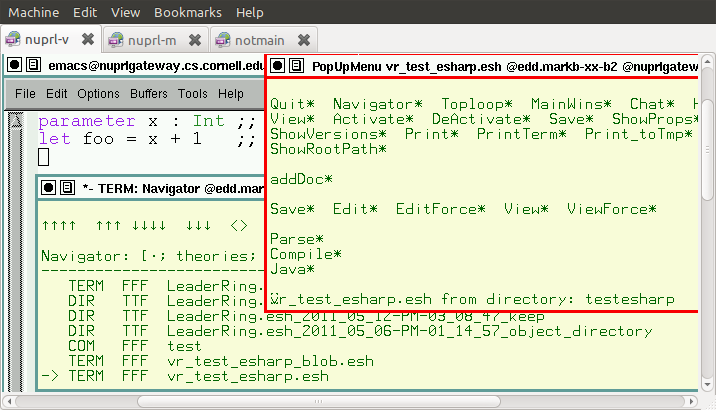
\includegraphics[width=0.9\textwidth]{../images/Esharp-test}
  \end{center}
  \caption{\eml\ blob within \nuprl}
  \label{fig:esharp-test}
\end{figure}

Clicking on the ``Compile'' button in the top right window, invokes
the \eml\ compiler and generates, among other things, two objects
(see Fig.~\ref{fig:esharp-test-compile}): (1) an abstraction
corresponding to foo's declaration (window marked ``ABS''), and a
well-formedness lemma (window marked ``PRF''), which is proved
automatically using a tactic called ``ProveWfLemma$\char19$''.

\begin{figure}[!t]
  \begin{center}
    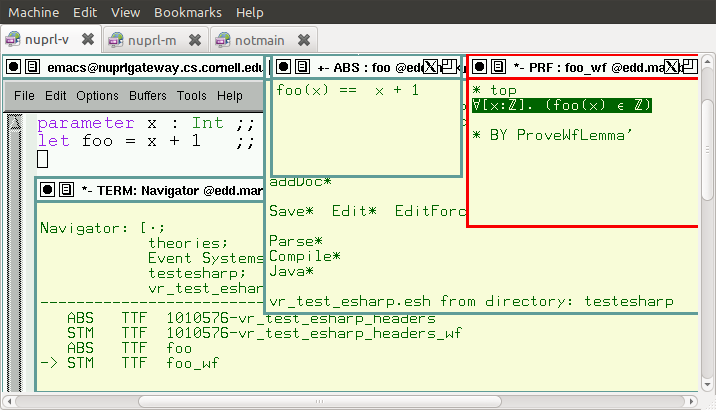
\includegraphics[width=0.9\textwidth]{../images/Esharp-test-compile}
  \end{center}
  \caption{Objects generated from \eml\ within \nuprl}
  \label{fig:esharp-test-compile}
\end{figure}


\subsection{Type error slicing}
\label{sec:tes}


\eml\ uses the type error
machinery~\cite{Haack+Wells:2003,Haack+Wells:2004,Rahli:2011} to
report type errors as well as to report syntax errors.  A type error
in an untypable piece of code is defined as a location set in the
piece of code that contains all and only the information necessary to
fix the error, i.e., the parts of the code where changes can be made
to fix the code, leaving out the parts where changes cannot fix the
error.  Such a location set is called a slice and is guaranteed (it is
at this stage only a conjecture as no formal proof as yet been
provided) to contain the user programming error.  We have an
\emacs\ interface that highlights slices directly in the source code.



\section{Examples}


Even though at this stage we haven't yet defined \eml's syntax (see
Sec.~\ref{sec:syntax}) and semantics (see Sec.~\ref{sec:semantics}),
we believe this section will help the reader get a feel of \eml.


\subsection{Leader election in a ring}


Leader election in general can be defined as the process of getting a
set of nodes (processes/agents) to agree on a unique leader.  A
particular case of such ``election'' distributed algorithms are when
nodes are arranged in a ring, where each node can only send messages
to its successor in the ring.
%
We have formalized leader election in a ring in \eml.
%
Let us present the different parts of this specification.
%
We divide the code in five parts: (1) parameters (see
Fig.~\ref{fig:LR_parameters}), (2) constants (see
Fig.~\ref{fig:LR_constants}), (3) type abbreviations (see
Fig.~\ref{fig:LR_typefunctions}), (4) message kind declarations (see
Fig.~\ref{fig:LR_messages}), and (5) the actual specification (see
Fig.~\ref{fig:LR_spec}).

\begin{figure}[!t]
  \begin{center}
\begin{lstlisting}
  parameter nodes  : Loc Bag ;;
  parameter client : Loc ;;
  parameter uid    : Loc -> Int ;;
\end{lstlisting}
  \end{center}
  \caption{Specification of the leader election in a ring in \eml: parameters}
  \label{fig:LR_parameters}
\end{figure}

\begin{figure}[!t]
  \begin{center}
\begin{lstlisting}
  constant imax (a : Int; b : Int) : Int ;;
\end{lstlisting}
  \end{center}
  \caption{Specification of the leader election in a ring in \eml: constants}
  \label{fig:LR_constants}
\end{figure}

\begin{figure}[!t]
  \begin{center}
\begin{lstlisting}
  type Epoch = Int ;;
\end{lstlisting}
  \end{center}
  \caption{Specification of the leader election in a ring in \eml: type functions}
  \label{fig:LR_typefunctions}
\end{figure}

\begin{figure}[!t]
  \begin{center}
\begin{lstlisting}
MSGS
  input    (``config`` : Epoch * Loc,
                base : Config @ nodes)
  (* Inform a node of its epoch and neighbor *)

  input    (``choose`` : Epoch,
                base : Choose @ nodes)
  (* Start the leader election *)

  output   (``leader`` : Epoch * Loc,
      	       	send : send_leader)
  (* Location of the leader *)

  internal (``propose`` : Epoch * Int,
                base : Propose @ nodes,
      	       	send : send_propose)
  (* Propose a node as the ring leader *)
;;
\end{lstlisting}
  \end{center}
  \caption{Specification of the leader election in a ring in \eml: message kinds}
  \label{fig:LR_messages}
\end{figure}

\begin{figure}[!t]
  \begin{center}
\begin{lstlisting}
let dumEpoch = 0 ;;

let Nbr =
  let f (epoch, succ) (epoch', succ') =
    if epoch > epoch'
    then (epoch, succ)
    else (epoch', succ') in
  f^|Config;Prior(self)?(\l.{(dumEpoch,l)})| ;;

let infix REPLY class F = F@|Loc;Prior(Nbr);class| ;;

let ProposeReply =
  let F loc (epoch, succ) (epoch', ldr) =
    if epoch = epoch'
    then if ldr = uid loc
         then {send_leader client (epoch, loc)}
         else {send_propose
                  succ
                  (epoch, imax ldr (uid loc))}
    else {}
  in Propose REPLY F ;;

let ChooseReply =
  let F loc (epoch, succ) epoch' =
    if epoch = epoch'
    then {send_propose succ (epoch, uid loc)}
    else {}
  in Choose REPLY F ;;

let LeaderRing = ProposeReply || ChooseReply ;;

main LeaderRing
\end{lstlisting}
  \end{center}
  \caption{Specification of the leader election in a ring in \eml}
  \label{fig:LR_spec}
\end{figure}

Let us describe the different classes defined in
Fig.~\ref{fig:LR_spec}.  \incodebody{Nbr} specifies a class of pairs
epoch/location.  This class is used to observe nodes' epochs an
successors.  The epoch and successor (called a state) of a node are
updated upon reception of a ``config'' message provided that the
node's current epoch precedes the new state's epoch.
%
The class \incodebody{PNbr} is used to observe the most recent state
of a node.

The \incodebody{REPLY} operator is used to define observers of replies
to events depending on the state of the node performing the reply.

The class \incodebody{ProposeReply} is used to observe the replies to
``propose'' events, i.e., the nodes' replies upon reception of
``propose'' messages.  If a node receives a ``propose'' message that
proposes itself as the leader, the node notifies the client that it
has been chosen as the leader.  Otherwise, the node sends a new
proposition to its successor.

The class \incodebody{ChooseReply} is used to observe the replies to
``choose'' events, i.e., the nodes' replies upon reception of
``choose'' messages.  Such messages are sent by the leader to start
the leader election.  If a node receives a ``choose'' message, it
proposes itself to its successor.

Finally, the class \incodebody{LeaderRing} is used to observe the
different events composing the leader election.


\subsection{Other examples}


We have started specifying the simple 2/3 consensus and are planning
on tackling leader election in a tree and Paxos.

%% \subsection{Leader election in a tree}

%% \fxnote{(2011-05-13) Empty section}

%% \subsection{Simple 2/3 consensus}

%% \fxnote{(2011-05-13) Empty section}

%% \subsection{Paxos}

%% \fxnote{(2011-05-13) Empty section}


\section{Notations and definitions}


%\smallintitle{Natural numbers}
%
Let $i, j, m, n, p, q$ be
metavariables ranging over $\SETnat$, the set of natural numbers.
%
%
%\smallintitle{Metavariables}
%
If a metavariable $v$ ranges over a class $\METAclass$, then the
metavariables $v_{x}$ (where $x$ can be anything) and the
metavariables $v', v''$, etc., also range over $\METAclass$.
%
%
%\smallintitle{Sets}
%
Let $\METAset$ range over sets.  If $v$ ranges over $\METAset$, then
let $\METAtoset{v}$ range over $\MEMpowset{\METAset}$, the power set
of $\METAset$.
%Let $\MEMsize{\METAs}$ be the cardinality of a set $\METAs$.
%
%
%
%\smallintitle{Disjunction}
%
Let $\MEMdisj{s_1,\dots,s_n}$ (``disjoint'') hold iff for all
$i,j\in\{1,\dots,n\}$, if $i\not=j$ then $s_i\cap{s_j}=\emptyset$.
%
Let $\MEMdunion{s_1}{s_2}$ be $s_1\cup{s_2}$ if $\MEMdisj{s_1,s_2}$ and
undefined otherwise.
%
%
%\smallintitle{Relations}
%
Let $\MEMpair{x}{y}$ be the pair of $x$ and $y$.
%
If $\METArel$ is a binary relation (a pair set),
%
let $(\MEMbrel{x}{\METArel}{y})$ iff $\MEMpair{x}{y}\in\METArel$,
%
let the inverse of $\METArel$ be
$\MEMinverse{\METArel}$ defined as
$\{\MEMpair{x}{y}\mid\MEMpair{y}{x}\in\METArel\}$,
let $\MEMdom{\METArel}=\{x\mid\MEMpair{x}{y}\in\METArel\}$,
let $\MEMran{\METArel}=\{y\mid\MEMpair{x}{y}\in\METArel\}$,
%
let
$\MEMrestrictin{\METArel}{s}=\{\MEMpair{x}{y}\in\METArel\mid{x}\in{s}\}$,
and let
$\MEMrestrictout{\METArel}{s}=\{\MEMpair{x}{y}\in\METArel\mid{x}\not\in{s}\}$.
%
%
%\smallintitle{Functions}
%
Let $\METAfun$ range over functions (a special case of binary relations),
let $\MEMfunc{s}{s'}=
\{\METAfun\mid\MEMdom{\METAfun}\subseteq{s}\wedge\MEMran{\METAfun}\subseteq{s'}\}$,
%% let $\MEMfunci{\METAs}{\METAs'}$ be $\MEMfunc{\METAs}{\METAs'}$ restricted to
%% injective functions,
and let $\asgn{x}{y}$ be
an alternative notation for $\MEMpair{x}{y}$ used when
writing some functions.
%
Let $\MEMuplus{\METAfun_1}{\METAfun_2}=\METAfun_2\cup(\MEMrestrictout{\METAfun_1}{\MEMdom{\METAfun_2}})$.
%
%Let $\METAfun_1,\METAfun_2\in\MEMfunc{s_1}{s_2}$.
Let
$\MEMequnion{\METAfun_1}{\METAfun_2}$ be $\METAfun_1\cup\METAfun_2$ if
$\METAfun_1\cup\METAfun_2$ is a function
and undefined otherwise.
%
If $\METAfun_1,\METAfun_2\in\MEMfunc{s_1}{\MEMpowset{s_2}}$ then let
$\MEMuenv{\METAfun_1}{\METAfun_2}
=\{\asgn{x}{\METAfun_1\cup\METAfun_2}\mid{x}\in\MEMdom{\METAfun_1}\cap\MEMdom{\METAfun_2}\}
\cup
\MEMrestrictout{\METAfun_1}{\MEMdom{\METAfun_2}}
\cup
\MEMrestrictout{\METAfun_2}{\MEMdom{\METAfun_1}}$.
%
%% Let
%% $\MEMfdunion{\METAfun_1}{\METAfun_2}=\METAfun_1\cup\METAfun_2$
%% if $\MEMdisj{\MEMdom{\METAfun_1},\MEMdom{\METAfun_2}}$
%% and undefined otherwise.
%
%
%
%\smallintitle{Tuples}
%
A tuple $\METAtup$ is a function such that $\MEMdom{\METAtup} \subset
\SETnat$ and if $1 \leq j \in \MEMdom{\METAtup}$ then $j - 1
\in \MEMdom{\METAtup}$.
%
Let $\METAtup$ range over tuples.
%
If $v$ ranges over $s$ then let $\METAtoseq{v}$ range
over $\MEMfintuple{s}=\{\METAtup\mid\MEMran{\METAtup}\subseteq{s}\}$.
%
We write the tuple
$\{\asgn{0}{x_0},\dots,\asgn{n}{x_n}\}$ as
$\mytuple{x_0,\dots,x_n}$.
%% We say that
%% $\mytuple{\METAx_1,\dots,\METAx_\METAn}$ is a
%% % finite
%% tuple of length $n$.
Let $@$ append tuples:
$\mytuple{x_1,\dots,x_i}@\mytuple{y_1,\dots,y_j}
=\mytuple{x_1,\dots,x_i,y_1,\dots,y_j}$.
%% $\mytuple{\METAx_1, \dots, \METAx_\METAn}$ and
%% $\mytuple{\METAy_1,\dots,\METAy_\METAm}$
%  Given a set $\METAs$, let $\MEMfintuple{\METAs} =
% \{\METAtup \mid \MEMran{\METAtup} \subseteq \METAs\}$.
%Given a set $\METAs$, let
%$\MEMfintuple{\METAs}=\{\METAtup\mid\MEMran{\METAtup}\subseteq\METAs\}$.
% \wedge \METAtup \mbox{ is a
%   finite tuple }\}$.
%% We use $\mytuple{}$ for
%% the empty tuple, i.e., $\mytuple{}$ is an alternative notation for
%% $\emptyset$ used when writing tuples.
%% We sometimes write $x\in\METAtoseq{\METAv}$ for $x\in\MEMran{\METAtoseq{\METAv}}$.
%
Given $n$ sets $s_1,\dots,s_n$, let $s_1\cprod\cdots\cprod{s_n}$ be
$\{\mytuple{x_1,\dots,x_n}\mid\forallexp{i\in\{1,\dots,n\}}{x_i\in{s_i}}\}$.
Note that
$s_1\cprod\cdots\cprod{s_n}\subseteq\MEMfintuple{s_1\cup\cdots\cup{s_n}}$.
%
%
%\smallintitle{Inference rules}
%
%% We often write our inference rules as follows:
%% $\MEMinferdd{x}{y_1}{\cdots}{y_n}{(r)}$, instead of the more
%% traditional form:
%% \begin{center}
%%   \begin{\sizeintables}
%%     $\infer[\MEMalgorule{r}]{x}{y_1 & \cdots & y_n}$
%%   \end{\sizeintables}
%% \end{center}
%
%% An inference rule is a pair premises/conclusion which states that if
%% the premises are true then the conclusion must be true as well.
%% %
%% In the literature, an inference rule is often written as follows:
%% \begin{center}
%%   \begin{\sizeintables}
%%     $\infer[\MEMalgorule{r}]{x}{y_1 & \cdots & y_n}$
%%   \end{\sizeintables}
%% \end{center}
%% which means that if $y_i$ for all $i\in\{1,\dots,n\}$ are true then
%% $x$ is true.
%% %
%% This rule is named $\MEMalgorule{r}$.
%% %
%% Such a rule is sometimes written as follows:
%% \begin{center}
%%   \begin{\sizeintables}
%%     $\MEMinferddr{x}{y_1}{\cdots}{y_n}{(r)}$
%%   \end{\sizeintables}
%% \end{center}
%% In this document we also sometimes write such a rule as follows:
%% \begin{center}
%%   \begin{\sizeintables}
%%     $\MEMinferdd{x}{y_1}{\cdots}{y_n}{(r)}$
%%   \end{\sizeintables}
%% \end{center}
%% %% or as follows:
%% %% \begin{center}
%% %%   \begin{\sizeintables}
%% %%     $(r)$ if $y_1$ and $\cdots$ and $y_n$ then $x$
%% %%   \end{\sizeintables}
%% %% \end{center}
%% The rule name is sometimes omitted in such rules.



\section{\eml's syntax}
\label{sec:syntax}


\fxnote{(2011-05-26) The optional syntax thing is undefined.}

\begin{figure}[t]
\begin{small}
\begin{center}
  \begin{tabular}{lllrl}
    $\METAint$
    & $\in$
    & $\SETint$
    & $=$
    & $\{\sim n \mid n \in \nat\}\cup\nat$
    \\

    $\METAatom$
    & $\in$
    & $\SETatom$
    &
    & (set of quoted strings without space)
    \\

    $\METAbool$
    & $\in$
    & $\SETbool$
    & $=$
    & $\CONStrue\mid\CONSfalse$
    \\

    $\METAop$
    & $\in$
    & $\SETop$
    & $::=$
    & $\CONSopplus
    \mid\CONSopminus
    \mid\CONSopequal
    \mid\CONSopeqequal
    \mid\CONSopdiff
    \mid\CONSoplistcons
    \mid\CONSople
    \mid\CONSoplt
    \mid\CONSopge
    \mid\CONSopgt$
    \\

    $\METAvid$
    & $\in$
    & $\SETvid$
    &
    & (an infinite countable set of value identifiers)
    \\

    $\METAeqtyvar$
    & $\in$
    & $\SETeqtyvar$
    &
    & (an infinite countable set of equality type variables)
    \\

    $\METAtyvar$
    & $\in$
    & $\SETtyvar$
    & $=$
    & (an infinite countable set of type variables
    \\
    &&&&
    \hspace*{0.05in}such that $\SETeqtyvar\subset\SETtyvar$)
    \\

    %% $\METAparam$
    %% & $\in$
    %% & $\SETparam$
    %% &
    %% & (an infinite countable set of type parameters)
    %% \\

    $\METAtycon$
    & $\in$
    & $\SETtycon$
    & $=$
    & (an infinite countable set of type constructors)
  \end{tabular}
\end{center}
\caption{\eml\ syntax - atomic terms}
\label{fig:esharp-syntax-atoms}
\end{small}
\end{figure}

\begin{figure}[t]
\begin{small}
\begin{center}
  \begin{tabular}{lllrl}
    $\METAatoms$
    & $\in$
    & $\SETatoms$
    & $::=$
    & $\CONSlistn{\METAatom_0}{\METAatom_n}$
    \\

    $\METAatomsl$
    & $\in$
    & $\SETatomsl$
    & $::=$
    & $\CONSvoid\mid\CONSatomsln{\METAatoms_0}{\METAatoms_n}$
    \\

    $\METAatexp$
    & $\in$
    & $\SETatexp$
    & $::=$
    & $\CONSopope{\METAvid}
    \mid\METAint
    \mid\METAatom
    \mid\METAbool$
    \\
    &&& $\mid$
    & $\CONSquotient{\METAexp}$
    \\
    &&& $\mid$
    & $\CONStupn{\METAexp_1}{\METAexp_n}$
    \\
    &&& $\mid$
    & $\CONSlistn{\METAexp_1}{\METAexp_n}$
    \\
    &&& $\mid$
    & $\CONSbagn{\METAexp_1}{\METAexp_n}$
    \\
    &&& $\mid$
    & $\CONSprior{\METAexp}$
    \\
    &&& $\mid$
    & $\CONSbase{\METAatomsl}{\METAexp}$
    \\
    &&& $\mid$
    & $\CONSmsg{\METAatoms}{\METAexp}$
    \\
    &&& $\mid$
    & $\CONSget{\METAatoms}$
    \\

    %% $\METAcrule$
    %% & $\in$
    %% & $\SETcrule$
    %% & $::=$
    %% & $\CONSmrulemsg{\METAmsgpat}{\METAexp}$
    %% \\

    %% $\METAbrule$
    %% & $\in$
    %% & $\SETbrule$
    %% & $::=$
    %% & $\CONSmrulebag{\METAbagpat}{\METAexp}$
    %% \\

    $\METAmrule$
    & $\in$
    & $\SETmrule$
    & $::=$
    & $\CONSmrule{\METAcasepat}{\METAexp}$
    \\

    $\METAexp$
    & $\in$
    & $\SETexp$
    & $::=$
    & $\METAatexp$
    \\
    &&& $\mid$
    & $\CONSopexp{\METAexp_1}{\METAop}{\METAexp_2}$
    %% \\
    %% &&& $\mid$
    %% & $\CONStexp{\METAty}$
    \\
    &&& $\mid$
    & $\CONStypexp{\METAexp}{\METAty}$
    \\
    &&& $\mid$
    & $\CONSappexp{\METAexp}{\METAatexp}$
    \\
    &&& $\mid$
    & $\CONSlamexp{\METApat}{\METAexp}$
    \\
    &&& $\mid$
    & $\CONSiteexp{\METAexp_1}{\METAexp_2}{\METAexp_3}$
    \\
    &&& $\mid$
    & $\CONSbindingexp{\METAexp_1}{\METApat}{\METAexp_2}$
    \\
    &&& $\mid$
    & $\CONSopjoinexpn{\METAatexp}{\METAatexp_0}{\METAatexp_n}$
    \\
    &&& $\mid$
    & $\CONSopjoinsexpn{\METAatexp}{\METAatexp_1}{\METAatexp_n}$
    %% \\
    %% &&& $\mid$
    %% & $\CONSjoinlexpn{\METAatexp}{\METAatexp_0}{\METAatexp_n}$
    %% \\
    %% &&& $\mid$
    %% & $\CONSjoinlsexpn{\METAatexp}{\METAatexp_1}{\METAatexp_n}$
    \\
    &&& $\mid$
    & $\CONSlet{\METAbind}{\METAexp}$
    \\
    &&& $\mid$
    & $\CONSletrec{\METAbind}{\METAexp}$
    \\
    &&& $\mid$
    & $\CONScaseexp{\METAexp}{\CONScasen{\METAmrule_0}{\METAmrule_n}}$
    \\
    %% &&& $\mid$
    %% & $\CONScasemsg{\METAexp}{\CONSmatchmsgn{\METAcrule_0}{\METAcrule_n}}$
    %% \\
    %% &&& $\mid$
    %% & $\CONScasebag{\METAexp}{\CONSmatchbagn{\METAbrule_0}{\METAbrule_n}}$
    %% \\
    %% &&& $\mid$
    %% & $\CONSmatchexp{\METAexp}{\CONSmatchn{\METAmrule_0}{\METAmrule_n}}$
  \end{tabular}
\end{center}
\caption{\eml\ syntax - expressions}
\label{fig:esharp-syntax-expressions}
\end{small}
\end{figure}

\begin{figure}[t]
\begin{small}
\begin{center}
  \begin{tabular}{lllrl}
    %% $\METAmsgpat$
    %% & $\in$
    %% & $\SETmsgpat$
    %% & $::=$
    %% & $\CONSmsgpat{\METAatoms}{\METApat}\mid\CONSwild$
    %% \\

    %% $\METAbagpat$
    %% & $\in$
    %% & $\SETbagpat$
    %% & $::=$
    %% & $\CONSbagpatnil\mid\CONSbagpatsing{\METAvid}\mid\CONSwild$
    %% \\

    $\METAcasepat$
    & $\in$
    & $\SETcasepat$
    & $::=$
    & $\CONSbagpatnil$
    \\
    &&& $\mid$
    & $\CONSbagpatsing{\METAvid}$
    \\
    &&& $\mid$
    & $\CONSmsg{\METAatoms}{\METApat}$
    \\
    &&& $\mid$
    & $\METApat$
    \\

    $\METAatpat$
    & $\in$
    & $\SETatpat$
    & $::=$
    & $\METAvid
    \mid\METAint
    \mid\METAatom
    \mid\METAbool
    \mid\CONSwild$
    \\
    &&& $\mid$
    & $\CONStupn{\METApat_1}{\METApat_n}$
    \\
    &&& $\mid$
    & $\CONSlistn{\METApat_1}{\METApat_n}$
    \\

    $\METApat$
    & $\in$
    & $\SETpat$
    & $::=$
    & $\METAatpat$
    \\
    &&& $\mid$
    & $\CONStyppat{\METApat}{\METAty}$
    \\
    &&& $\mid$
    & $\CONSoplistpat{\METApat_1}{\METApat_2}$
  \end{tabular}
\end{center}
\caption{\eml\ syntax - patterns}
\label{fig:esharp-syntax-patterns}
\end{small}
\end{figure}

\begin{figure}[t]
\begin{small}
\begin{center}
  \begin{tabular}{lllrl}
    $\METAtypseq$
    & $\in$
    & $\SETtypseq$
    & $::=$
    & $\CONSvoid$
    \\
    &&& $\mid$
    & $\METAty$
    \\
    &&& $\mid$
    & $(\METAty_0,\dots,\METAty_n)$
    \\

    $\METAty$
    & $\in$
    & $\SETty$
    & $::=$
    & $\METAtyvar$
    \\
    &&& $\mid$
    & $\CONSconsty{\METAtypseq}{\METAtycon}$
    \\
    &&& $\mid$
    & $\CONSdisjuty{\METAty_1}{\METAty_2}$
    \\
    &&& $\mid$
    & $\CONSarrowty{\METAty_1}{\METAty_2}$
    \\
    %% &&& $\mid$
    %% & $\CONSdepty{\METAvid}{\METAty}$
    %% \\
    &&& $\mid$
    & $\CONStuptyn{\METAty_0}{\METAty_n}$
    \\
    &&& $\mid$
    & $(\METAty)$
  \end{tabular}
\end{center}
\caption{\eml\ syntax - types}
\label{fig:esharp-syntax-types}
\end{small}
\end{figure}


\begin{figure}[t]
\begin{small}
\begin{center}
  \begin{tabular}{lllrl}
    $\METAtypvarseq$
    & $\in$
    & $\SETtypvarseq$
    & $::=$
    & $\CONSvoid$
    \\
    &&& $\mid$
    & $\METAtyvar$
    \\
    &&& $\mid$
    & $(\METAtyvar_0,\dots,\METAtyvar_n)$
    \\

    $\METAtypseqset$
    & $\in$
    & $\SETtypseqset$
    & $::=$
    & $\CONStypseqsetn{\METAtypseq_1}{\METAtypseq_n}$
    \\

    $\METAbind$
    & $\in$
    & $\SETbind$
    & $::=$
    & $\CONSbindpat{\METApat}{\METAexp}$
    \\
    &&& $\mid$
    & $\CONSbindappopty{\METAvid}{\CONSparamn{\METAatpat_0}{\METAatpat_n}}{\METAty}{\METAexp}$
    \\
    &&& $\mid$
    & $\CONSbindinfixopty{\METAvid}{\METApat_1}{\METApat_2}{\METAty}{\METAexp}$
    \\
    &&& $\mid$
    & $\CONSbindinfixropty{\METAvid}{\METApat_1}{\METApat_2}{\METAty}{\METAexp}$
    \\

    $\METAbvars$
    & $\in$
    & $\SETbvars$
    & $::=$
    & $\CONSbvarsn{\CONSonebvar{\METAvid_1}{\METAty_1}}{\CONSonebvar{\METAvid_n}{\METAty_n}}$
    \\

    $\METAarg$
    & $\in$
    & $\SETarg$
    & $::=$
    & $\CONSoneargop{\METAvid}{\METAty}{\METAbvars}$
    \\

    $\METAargs$
    & $\in$
    & $\SETargs$
    & $::=$
    & $\CONSargsn{\METAarg_1}{\METAarg_n}$
    \\

    $\METAheader$
    & $\in$
    & $\SETheader$
    & $::=$
    & $\CONSheadert{\METAatoms}{\METAty}$
    \\
    &&& $\mid$
    & $\CONSheaderc{\METAvid}{\METAatoms}{\METAty}$
    \\
    &&& $\mid$
    & $\CONSheaderl{\METAvid}{\METAexp}{\METAatoms}{\METAty}$
    \\

    $\METAdec$
    & $\in$
    & $\SETdec$
    & $::=$
    & $\CONSletdec{\METAbind}$
    \\
    &&& $\mid$
    & $\CONSletrecdec{\METAbind}$
    \\
    &&& $\mid$
    & $\CONSconsOpargsOpovOpcsDec{\METAvid}{\METAargs}{\METAty}{\METAtypvarseq}{\METAtypseqset}{\METAexp}$
    \\
    &&& $\mid$
    & $\CONSparameter{\METAvid}{\METAty}$
    \\
    &&& $\mid$
    & $\CONSconstydecOpeq{\METAtypvarseq}{\METAtycon}{\METAvid}$
    \\
    &&& $\mid$
    & $\CONSparameterOpeq{\METAtypvarseq}{\METAtycon}{\METAvid}$
    %% \\
    %% &&& $\mid$
    %% & $\CONStypedec{\METAtypvarseq}{\METAtycon}$
    %% \\
    %% &&& $\mid$
    %% & $\CONSeqtypedec{\METAtypvarseq}{\METAtycon}$
    \\
    &&& $\mid$
    & $\CONStypefundec{\METAtypvarseq}{\METAtycon}{\METAty}$
    \\
    &&& $\mid$
    & $\CONSmsgsdecn{\METAheader_1}{\METAheader_n}$
    \\

    $\METAprog$
    & $\in$
    & $\SETprog$
    & $::=$
    & $\CONSprogem$
    \\
    &&& $\mid$
    & $\CONSprog{\CONSdec{\METAdec}}{\METAprog}$
  \end{tabular}
\end{center}
\caption{\eml\ syntax - binders and declarations}
\label{fig:esharp-syntax-declarations}
\end{small}
\end{figure}


Fig.~\ref{fig:esharp-syntax-atoms},
\ref{fig:esharp-syntax-expressions},
\ref{fig:esharp-syntax-patterns},
\ref{fig:esharp-syntax-types},
and~\ref{fig:esharp-syntax-declarations}, presents \eml's syntax.
Following the syntax used by \SML, we use $\CONS{(*}$ and $\CONS{*)}$
to delimit comments.
%
Type variables are identifiers preceded with a single quote.
%
\eml\ has the following builtin nullary type constructors:
$\{\CONSintty,\CONSmsgty,\CONSboolty,\CONSunitty,\CONSatomty,\CONSlocty\}
\subset\SETtycon$, and the following builtin unary type constructors:
$\{\CONSclassty,\CONSbagty,\CONSlistty\}\subset\SETtycon$.

\fxnote{(2011-05-13) We also have the $\CONSnatty$ type but it is
  currently useless because we don't have subtyping and $1$, $2$,
  \dots\ all have type $\CONSintty$.  Also $+$, $-$, \dots\ take
  integers.}

\fxnote{(2011-05-13) I need to add $\CONSdeqty$ to the list of unary
  type constructors.}

\fxnote{(2011-05-13) We also consider the nullary constructor
  $\CONStypety$ but only allow it in certain declarations.}

%% \fxnote{(2011-03-04) We should be able to define also non-nullary
%%   constructors with the 'type' declarations.}


\subsection{Syntactic sugar}

Atom lists of the form $\CONSlistn{\METAatom_0}{\METAatom_n}$ can
be written using backquotes as follows: $\CONSatomsn{\METAatom_0}{\METAatom_n}$.
%
Expressions of the form
$\CONSbindingexp{\METAexp_1}{\METApat}{\METAexp_2}$ can be written
using the \haskell\ monodic bind operator as follows:
$\CONSmonbindexp{\METAexp_1}{\CONSlamexp{\METApat}{\METAexp_2}}$.



\subsection{\eml's declarations}
\label{sec:esharp-declarations}


Declarations of the form $\CONSletdec{\METAbind}$ and
$\CONSletrecdec{\METAbind}$ are used to declare non-recursive and
recursive identifiers respectively.  $\CONS{constant}$ declarations are
used to import \nuprl\ abstractions.  Let us explain the $\METAargs$
part of such declarations.  \nuprl's abstractions (\nuprl's terms in
general) have arities.  The length of the $\METAargs$ part of a
$\CONS{constant}$ declaration gives the arity of the imported
abstraction.  One might sometimes make explicit variable bindings in
terms.  For example the existential quantifier is defined in
\nuprl\ as a dependent pair $x$ of type $A$ and a type $B$ in which
$x$ might occur.  The existential term is then defined as a binary
term.  It has two subterms which are: (1) a type A, and (2) a
binding of a variable $x$ in a type $B$.  This explains the part
$\METAbvars$ in a subterm specification of the form
$\CONSoneargbvars{\METAvid}{\METAty}{\METAbvars}$.
Providing a $\CONS{constant}$ declaration of the form
$\CONSconsargsdec
{f}
{\CONSargs
  {\CONSoneargbvars
    {b}
    {\METAty_2}
    {\CONSbvars
      {\CONSonebvar
        {x}
        {\METAty_1}
      }
    }
  }
}
{\METAty_3}$
instead of
$\CONSconsdec
{f}
{\CONSarrowty
  {(\CONSarrowty{\METAty_1}{\METAty_2})}
  {\METAty_3}
}$
allows generating the correct \nuprl\ terms for each of $f$'s uses in
a \eml\ piece of code.
%

Types can be imported from \nuprl\ using $\CONS{constant}$
declarations as follows:
$\CONSconstydecOpeq{\METAtypvarseq}{\METAtycon}{\METAvid}$.  A type
constructor $\METAtycon$ can either have equality (equality in a
type with top type constructor $\METAtycon$ is decidable provided that
it is decidable in its arguments) or not (equality is not decidable).
If a type constructor has equality it means that one can construct a
equality decider.  Therefore,
$\CONSconstyndeq{\METAtypvarseq}{\METAtycon}$ declares a type that
does not have equality, while
$\CONSconstydec{\METAtypvarseq}{\METAtycon}{\METAvid}$ declares a
type that has equality and where $\METAvid$ is one of its equality
decider.

An entire \eml\ program can be parametrized (using
$\CONS{parameter}$ declarations).  For example, one might want to
write the specification of the information flow of a distributed
system without committing to a specific locations for the system's
components.  One can then parametrize the specification by a location
list.

\eml\ allows declaring type function as follows:
$\CONStypefundec{\METAtypvarseq}{\METAtycon}{\METAty}$.  This is
useful, e.g., to provide type abbreviation.  Note that these
declarations are not exported to \nuprl.  Type functions are unfolded
during type inference.

$\CONS{MSGS}$ declarations are used to declare the different kinds of
messages used in by a distributed system.  A message is composed by a
header and a content of a certain type.  Declaring
$\CONSmsgsdec{\CONSheadert{\CONSatoms{\mbox{foo}}}{\CONSintty}}$ says
that some messages have header $\CONSatoms{\mbox{foo}}$ and content of
type $\CONSintty$.

\hidden{
Note that a type can be of the form $\CONSdepty{\METAvid}{\METAty}$
in order to be able to write declarations as follows:
\incodebody{cons hd : (x : 'a List) -> 'a | not (null x);;}.
\fxnote{(2011-03-08) We don't currently parse these forms.}
}


\subsection{Additional syntactic restrictions}

Additional syntactic restrictions on patterns:
\begin{itemize}
\item In $\CONSbindpat{\METApat}{\METAexp}$, no pattern of the form
  $\METAint$, $\METAatom$, $\METAbool$,
  $\CONSlistn{\METApat_1}{\METApat_n}$, or
  $\CONSoplistpat{\METApat_1}{\METApat_2}$,
  can occur in $\METApat$.
  The same restriction applies to the $\METAatpat_i$s
  in
  $\CONSbindappopty{\METAvid}{\CONSparamn{\METAatpat_0}{\METAatpat_n}}{\METAty}{\METAexp}$
  and to $\METApat$'s in
  $\CONSmsg{\METAatoms}{\METApat}$.
\end{itemize}

\noindent
Additional syntactic restrictions on expressions:
\begin{itemize}
%% \item
%%   In
%%   $\CONScasemsg{\METAexp}{\CONSmatchmsgn{\METAcrule_0}{\METAcrule_n}}$,
%%   $\METAcrule_n$ is of the form $\CONSmrulemsg{\CONSwild}{\METAexp}$,
%%   and for $i\in\{0,\dots,n-1\}$, $\METAcrule_i$ is of the form
%%   $\CONSmrulemsg{\METAmsgpat}{\METAexp}$ where $\METAmsgpat$ is not of
%%   the form $\CONSwild$.

%% \item
%%   Similarly, in
%%   $\CONScasebag{\METAvid}{\METAexp}{\CONSmatchbagn{\METAbrule_0}{\METAbrule_n}}$,
%%   $\METAbrule_n$ is of the form $\CONSmrulebag{\CONSwild}{\METAexp}$, and
%%   for $i\in\{0,\dots,n-1\}$, $\METAbrule_i$ is of the form
%%   $\CONSmrulebag{\METAbagpat}{\METAexp}$ where $\METAbagpat$ is not of the form
%%   $\CONSwild$.

\item
  In
  $\CONScaseexp{\METAvid}{\METAexp}{\CONScasen{\METAmrule_0}{\METAmrule_n}}$,
  one of these holds:
  \begin{itemize}
  \item $\METAmrule_n$ is of the form
    $\CONSmrule{\CONSwild}{\METAexp}$, and one of these holds:
    \begin{itemize}
    \item
      Each $\METAmrule_i$, for $i\in\{0,\dots,n-1\}$ are of the form
      $\CONSmsg{\METAatoms}{\METApat}$.
    \item
      $n=1$ and $\METAmrule_{0}$ is of the form
      $\CONSbagpatsing{\METAvid}$.
    \item
      $n=2$ and one $\METAmrule_i$, for $i\in\{0,1\}$ is of the form
      $\CONSbagpatsing{\METAvid}$ while the other is of the form
      $\CONSbagpatnil$.
    \end{itemize}
  \item $n=1$ and one $\METAmrule_i$, for $i\in\{0,1\}$ is of the form
    $\CONSemlist$ or $\CONSnil$ while the other is of the form
    $\CONSoplistpat{\METAvid_1}{\METAvid_2}$.
  \end{itemize}
\end{itemize}

\noindent
Additional syntactic restrictions on bindings and declarations:
\begin{itemize}
\item In
  $\CONSconsOpovOpcsDec{\METAvid}{\METAty}{\METAtypvarseq}{\CONStypseqsetn{\METAtypseq_1}{\METAtypseq_n}}{\METAexp}$:
  for all $i\in\{1,\dots,n\}$, $\METAtypseq_i$ cannot be $\CONSvoid$;
  $\METAtypvarseq$ cannot be $\CONSvoid$;
  for all $i\in\{1,\dots,n\}$, the arity of $\METAtypseq_i$ must be
  equal to the arity of $\METAtypvarseq$.

\item In $\CONSletrecdec{\CONSbindpat{\METApat}{\METAexp}}$,
  $\METApat$ has to be an identifier and $\METAexp$ a
  $\lambda$-abstraction.

\item In $\CONSconstydecOpeq{\METAtypvarseq}{\METAtycon}{\METAvid}$,
  $\CONSparameterOpeq{\METAtypvarseq}{\METAtycon}{\METAvid}$, or
  $\CONStypefundec{\METAtypvarseq}{\METAtycon}{\METAty}$, no type
  variable can occur twice in $\METAtypvarseq$, and in the last form
  each type variable occurring in $\METAty$ must occur in
  $\METAtypvarseq$.
\end{itemize}


%% \subsection{Requested features}

%% It would be useful to have
%% $\SETcrule::=\cdots\mid\CONSmrulemsg{\METAvid}{\METAexp}$.


\section{\eml's static semantics}
\label{sec:semantics}
% Typing rules

Fig.~\ref{fig:typing-rules-atomic-expressions},
\ref{fig:typing-rules-mrules},
\ref{fig:typing-rules-expressions},
\ref{fig:typing-rules-patterns},
\ref{fig:typing-rules-bindings},
and~\ref{fig:typing-rules-declarations}
presents \eml's static semantics.

First, let us define some syntax for internal types:
\begin{center}
  \begin{tabular}{lllrl}
    $\METAity$
    & $\in$
    & $\SETity$
    & $::=$
    & $\METAtyvar$
    \\
    &&& $\mid$
    & $\CONSconsty{\METAityseq}{\METAtycon}$
    \\
    &&& $\mid$
    & $\CONSdisjuty{\METAity_1}{\METAity_2}$
    \\
    &&& $\mid$
    & $\CONSarrowty{\METAity_1}{\METAity_2}$
    \\
    &&& $\mid$
    & $\CONStuptyn{\METAity_0}{\METAity_n}$
    \\

    $\METAityscheme$
    & $\in$
    & $\SETityscheme$
    & $::=$
    & $\CONSityschemeb{\METAtyvarset}{\METAity}$
    \\

    $\METAityfun$
    & $\in$
    & $\SETityfun$
    & $::=$
    & $\CONSityfun{\METAtyvarseq}{\METAity}$
    \\

    $\METAityenv$
    & $\in$
    & $\SETityenv$
    & $=$
    & $\{
    \METAfun
    \begin{array}[t]{ll}
      \mid
      &
      \METAfun
      =\METAfun_1
      \cup\METAfun_2
      \cup\METAfun_3
      \\
      \wedge
      &
      \METAfun_1\in\MEMfunc{\SETvid}{\SETtoset{\SETityscheme}}
      \\
      \wedge
      &
      \METAfun_2\in\MEMfunc{\SETatoms}{\SETityscheme}
      \\
      \wedge
      &
      \METAfun_3\in\MEMfunc{\SETtycon}{\SETityfun}\}
    \end{array}$
  \end{tabular}
\end{center}


In environment, we sometimes write $\METAity$ for the type scheme
$\CONSityschemeb{\emptyset}{\METAity}$.
%
We often write $\METAtycon$ for the internal type
$\CONSconsty{\mytuple{}}{\METAtycon}$.
%
We often write
$\{\asgn{\METAvid}{\METAityscheme}\}\cup\METAityenv$
for the environment
$\{\asgn{\METAvid}{\{\METAityscheme\}}\}\cup\METAityenv$.

%% The function $\MEMinternalTySYMB$ extracts an internal type from an
%% external one and the function $\MEMinternalTyseqSYMB$ extracts a
%% sequence of internal types from an external type sequence as follows:
%% \begin{center}
%%   \begin{tabular}{lll}
%%     \multicolumn{3}{l}{On types}
%%     \\

%%     $\MEMinternalTy{\METAtyvar}$
%%     & $=$
%%     & $\METAtyvar$
%%     \\

%%     $\MEMinternalTy{\CONSconsty{\METAtypseq}{\METAtycon}}$
%%     & $=$
%%     & $\CONSconsty{\MEMinternalTyseq{\METAtypseq}}{\METAtycon}$
%%     \\

%%     $\MEMinternalTy{\CONSdisjuty{\METAty_1}{\METAty_2}}$
%%     & $=$
%%     & $\CONSdisjuty{\MEMinternalTy{\METAty_1}}{\MEMinternalTy{\METAty_2}}$
%%     \\

%%     $\MEMinternalTy{\CONSarrowty{\METAty_1}{\METAty_2}}$
%%     & $=$
%%     & $\CONSarrowty{\MEMinternalTy{\METAty_1}}{\MEMinternalTy{\METAty_2}}$
%%     \\

%%     $\MEMinternalTy{\CONSdepty{\METAvid}{\METAty}}$
%%     & $=$
%%     & $\MEMinternalTy{\METAty}$
%%     \\

%%     $\MEMinternalTy{\CONStuptyn{\METAty_0}{\METAty_n}}$
%%     & $=$
%%     & $\CONStuptyn{\MEMinternalTy{\METAty_0}}{\MEMinternalTy{\METAty_n}}$
%%     \\

%%     $\MEMinternalTy{(\METAty)}$
%%     & $=$
%%     & $\MEMinternalTy{\METAty}$
%%     \\

%%     &&\\

%%     \multicolumn{3}{l}{On type sequences}
%%     \\

%%     $\MEMinternalTyseq{\CONSvoid}$
%%     & $=$
%%     & $\mytuple{}$
%%     \\

%%     $\MEMinternalTyseq{\METAty}$
%%     & $=$
%%     & $\mytuple{\MEMinternalTy{\METAty}}$
%%     \\

%%     $\MEMinternalTyseq{(\METAty_0,\dots,\METAty_n)}$
%%     & $=$
%%     & $\mytuple{\MEMinternalTy{\METAty_0},\dots,\MEMinternalTy{\METAty_n}}$
%%   \end{tabular}
%% \end{center}

Let the function $\MEMtypeofopSYMB$ be defined in operators as
follows:
\begin{center}
  \begin{tabular}{lll}
    $\MEMtypeofop{\CONSopplus}$
    & $=$
    & $\CONSityschemeb{\emptyset}{\CONSarrowty{\CONStupty{\CONSintty}{\CONSintty}}{\CONSintty}}$
    \\

    $\MEMtypeofop{\CONSopminus}$
    & $=$
    & $\CONSityschemeb{\emptyset}{\CONSarrowty{\CONStupty{\CONSintty}{\CONSintty}}{\CONSintty}}$
    \\

    $\MEMtypeofop{\CONSopequal}$
    & $=$
    & $\CONSityscheme{\METAeqtyvar}{\CONSarrowty{\CONStupty{\METAeqtyvar}{\METAeqtyvar}}{\CONSboolty}}$
    \\

    $\MEMtypeofop{\CONSopeqequal}$
    & $=$
    & $\CONSityscheme{\METAeqtyvar}{\CONSarrowty{\CONStupty{\METAeqtyvar}{\METAeqtyvar}}{\CONSboolty}}$
    \\

    $\MEMtypeofop{\CONSopdiff}$
    & $=$
    & $\CONSityscheme{\METAeqtyvar}{\CONSarrowty{\CONStupty{\METAeqtyvar}{\METAeqtyvar}}{\CONSboolty}}$
    \\

    $\MEMtypeofop{\CONSoplistcons}$
    & $=$
    & $\CONSityscheme{\METAtyvar}{\CONSarrowty{\CONStupty{\METAtyvar}{\CONSconsty{\METAtyvar}{\CONSlistty}}}{\CONSconsty{\METAtyvar}{\CONSlistty}}}$
  \end{tabular}
\end{center}

Substitutions are defined as follows:
\begin{center}
  \begin{tabular}{lllrl}
    $\METAsub$
    & $\in$
    & $\SETsub$
    & $=$
    & $\MEMfunc{\SETtyvar}{\SETity}$
  \end{tabular}
\end{center}

Substitutions are applied to internal types as follows:
\begin{center}
  \begin{tabular}{lll}
    $\MEMsub{\METAtyvar}{\METAsub}$
    & $=$
    & $\left\{
    \begin{array}{ll}
      \MEMafunc{\METAsub}{\METAtyvar},
      &
      \mbox{if }\METAtyvar\in\MEMdom{\METAsub}
      \\
      \METAtyvar,
      &
      \mbox{otherwise}
    \end{array}
    \right.$
    \\

    $\MEMsub{(\CONSconsty{\mytuple{\METAity_1,\dots,\METAity_n}}{\METAtycon})}{\METAsub}$
    & $=$
    & $\CONSconsty{\mytuple{\MEMsub{\METAity_1}{\METAsub},\dots,\MEMsub{\METAity_n}{\METAsub}}}{\METAtycon}$
    \\

    $\MEMsub{(\CONSdisjuty{\METAity_1}{\METAity_2})}{\METAsub}$
    & $=$
    & $\CONSdisjuty{\MEMsub{\METAity_1}{\METAsub}}{\MEMsub{\METAity_n}{\METAsub}}$
    \\

    $\MEMsub{(\CONSarrowty{\METAity_1}{\METAity_2})}{\METAsub}$
    & $=$
    & $\CONSarrowty{\MEMsub{\METAity_1}{\METAsub}}{\MEMsub{\METAity_2}{\METAsub}}$
    \\

    $\MEMsub{(\CONStuptyn{\METAity_1}{\METAity_n})}{\METAsub}$
    & $=$
    & $\CONStuptyn{\MEMsub{\METAity_1}{\METAsub}}{\MEMsub{\METAity_n}{\METAsub}}$
  \end{tabular}
\end{center}
%% \fxnote{(2011-03-08) Do we really have the internal types to the
%%   external ones.  It means that the above definition is incomplete
%%   because we don't have the parentheses case.  Also we don't have the
%%   dependent case.}

Let the instantiation of a type scheme be defined as follows:
\begin{center}
  \begin{tabular}{l}
    $\MEMinstance{\METAity}{\CONSityscheme{\METAtyvar_1,\dots,\METAtyvar_n}{\METAity'}}$
    $\iff$
    $\existsexp
    {\METAity_1,\dots,\METAity_n}
    {\METAity
      =\MEMsub
      {\METAity'}
      {\{\asgn{\METAtyvar_i}{\METAity_i}\mid{i}\in\{1,\dots,n\}\}}
    }$
    \\

    $\MEMinstance{\METAity}{\METAityschemeset}$
    $\iff$
    $\existsexp
    {\METAityscheme\in\METAityschemeset}
    {\MEMinstance{\METAity}{\METAityscheme}}$
  \end{tabular}
\end{center}

The free type variables of internal types and type environments are
defined as follows:
\begin{center}
  \begin{tabular}{lll}
    $\MEMfreetyvars{\METAityenv}$
    & $=$
    & $\{\METAtyvar
    \mid
    \CONSityschemeb{\METAtyvarset}{\METAity}\in\MEMafunc{\METAityenv}{\METAvid}
    \wedge
    \METAtyvar\in\MEMfreetyvars{\METAity}\setminus\METAtyvarset\}$
    \\

    $\MEMfreetyvars{\METAity}$
    & $=$
    & $\{\METAtyvar\mid\METAtyvar\mbox{ occurs in }\METAity\}$
  \end{tabular}
\end{center}

Let the closure of a type environment be defined as follows:
\begin{center}
  $\MEMclos{\METAityenv}{\METAityenv'}
  =\{\asgn{\METAvid}{\{\CONSityschemeb{(\MEMfreetyvars{\METAity}\setminus\MEMfreetyvars{\METAityenv})}{\METAity}\mid\METAity\in\METAityset\}}
  \mid
  \MEMafunc{\METAityenv'}{\METAvid}=\METAityset\}$
\end{center}

\fxnote{(2011-03-08) I also have to define the closure of the explicit
  type variables.}

\begin{center}
  \begin{tabular}{l}
    $\MEMoverload
    {\METAity}
    {\METAtyvar}
    {\mytuple{
        \mytuple{\METAity_1},
        \dots,
        \mytuple{\METAity_m}
      }
    }$
    \\
    \hspace*{0.2in}
    $=$
    $\{\MEMsub{\METAity}{\{\asgn{\METAtyvar}{\METAity_i}\}}
    \mid
    i\in\{1,\dots,m\}\}$
    \\

    $\MEMoverload
    {\METAity}
    {(\METAtyvar_0,\dots,\METAtyvar_n)}
    {\mytuple{
        \mytuple{\METAity^{1}_{1},\dots,\METAity^{m}_{1}},
        \dots,
        \mytuple{\METAity^{1}_{n},\dots,\METAity^{m}_{n}}
      }
    }$
    \\
    \hspace*{0.2in}
    $=$
    $\{\MEMsub{\METAity}{\{\asgn{\METAtyvar_1}{\METAity^{i}_{1}},\dots,\asgn{\METAtyvar_n}{\METAity^{i}_n}\}}
    \mid
    i\in\{1,\dots,m\}\}$
  \end{tabular}
\end{center}


\begin{figure}[t]
\begin{small}
\begin{center}
  \begin{tabular}{llll}
    $\MEMinferb
    {\MEMtyping{\METAvid}{\METAityenv}{\METAity}}
    {\MEMinstance{\METAity}{\MEMafunc{\METAityenv}{\METAvid}}}$

    &

    $\MEMinfera
    {\MEMtyping{\METAint}{\METAityenv}{\CONSintty}}$

    &

    $\MEMinfera
    {\MEMtyping{\METAatom}{\METAityenv}{\CONSatomty}}$

    &

    $\MEMinfera
    {\MEMtyping{\METAbool}{\METAityenv}{\CONSboolty}}$

    \\
    &&&
    \\

    \multicolumn{2}{l}{
      $\MEMinferb
      {\MEMtyping{\CONStupn{\METAexp_0}{\METAexp_n}}{\METAityenv}{\CONStuptyn{\METAity_0}{\METAity_n}}}
      {\forallexp{i\in\{0,\dots,n\}}{\MEMtyping{\METAexp_i}{\METAityenv}{\METAity_i}}}$
    }

    &

    \multicolumn{1}{l}{
      $\MEMinferb
      {\MEMtyping{\CONSquotient{\METAexp}}{\METAityenv}{\CONSconsty{\METAity}{\CONSbagty}}}
      {\MEMtyping{\METAexp}{\METAityenv}{\CONSconsty{\METAity}{\CONSlistty}}}$
    }

    &

    \multicolumn{1}{l}{
      $\MEMinfera
      {\MEMtyping{()}{\METAityenv}{\CONSunitty}}$
    }

    \\
    &&&
    \\

    \multicolumn{2}{l}{
      $\MEMinferb
      {\MEMtyping{\CONSlistn{\METAexp_1}{\METAexp_n}}{\METAityenv}{\CONSconsty{\METAity}{\CONSlistty}}}
      {\forallexp{i\in\{1,\dots,n\}}{\MEMtyping{\METAexp_i}{\METAityenv}{\METAity}}}$
    }

    &

    \multicolumn{2}{l}{
      $\MEMinferb
      {\MEMtyping{\CONSbagn{\METAexp_1}{\METAexp_n}}{\METAityenv}{\CONSconsty{\METAity}{\CONSbagty}}}
      {\forallexp{i\in\{1,\dots,n\}}{\MEMtyping{\METAexp_i}{\METAityenv}{\METAity}}}$
    }

    \\
    &&&
    \\

    \multicolumn{2}{l}{
      $\MEMinferb
      {\MEMtyping{\CONSprior{\METAexp}}{\METAityenv}{\CONSconsty{\METAity}{\CONSclassty}}}
      {\MEMtyping{\METAexp}{\METAityenv}{\CONSconsty{\METAity}{\CONSclassty}}}$
    }

    &

    \multicolumn{2}{l}{
      $\MEMinferb
      {\MEMtyping{\CONSbase{\METAatomsl}{\METAexp}}{\METAityenv}{\CONSconsty{\CONSmsgty}{\CONSclassty}}}
      {\MEMtyping{\METAexp}{\METAityenv}{\CONSconsty{\CONSlocty}{\CONSlistty}}}$
    }

    \\
    &&&
    \\

    \multicolumn{2}{l}{
      $\MEMinferc
      {\MEMtyping{\CONSmsg{\METAatoms}{\METAexp}}{\METAityenv}{\CONSmsgty}}
      {\MEMinstance{\METAity}{\MEMafunc{\METAityenv}{\METAatoms}}}
      {\MEMtyping{\METAexp}{\METAityenv}{\METAity}}$
    }

    &

    \multicolumn{2}{l}{
      $\MEMinferb
      {\MEMtyping{\CONSget{\METAatoms}}{\METAityenv}{\CONSarrowty{\CONSconsty{\CONSmsgty}{\CONSbagty}}{\CONSconsty{\METAity}{\CONSbagty}}}}
      {\MEMinstance{\METAity}{\MEMafunc{\METAityenv}{\METAatoms}}}$
    }
  \end{tabular}
\end{center}
\caption{\eml\ typing rules - atomic expressions}
\label{fig:typing-rules-atomic-expressions}
\end{small}
\end{figure}


\begin{figure}[t]
\begin{small}
\begin{center}
  \begin{tabular}{llllll}
    \multicolumn{2}{l}{
      $\MEMinferc
      {\MEMtypingpat{\CONSmsg{\METAatoms}{\METApat}}{\METAityenv}{\CONSmsgty}}
      {\MEMtyping{\METApat}{\METAityenv}{\METAity}}
      {\MEMinstance{\METAity}{\MEMafunc{\METAityenv}{\METAatoms}}}$
    }

    &

    \multicolumn{2}{l}{
      $\MEMinfera
      {\MEMtypingpat{\CONSbagpatsing{\METAvid}}{\{\asgn{\METAvid}{\METAity}\}}{\CONSconsty{\METAity}{\CONSbagty}}}$

    }

    %% \\
    %% &&&
    %% \\

    %% \multicolumn{2}{l}{
    %%   $\MEMinfera
    %%   {\MEMtypingpat{\CONSvoid}{\CONSemptyityenv}{\METAity}}$
    %% }

    &

    \multicolumn{2}{l}{
      $\MEMinfera
      {\MEMtypingpat{\CONSbagpatnil}{\CONSemptyityenv}{\CONSconsty{\METAity}{\CONSbagty}}}$
    }

    \\
    &&&
    \\

    %% \multicolumn{3}{l}{
    %%   $\MEMinferc
    %%   {\MEMtyping{\CONSmrulemsg{\METAmsgpat}{\METAexp}}{\METAityenv}{\CONSarrowty{\METAity_1}{\METAity_2}}}
    %%   {\MEMtypingpat{\METAmsgpat}{\METAityenv'}{\METAity_1}}
    %%   {\MEMtyping{\METAexp}{\MEMplusenv{\METAityenv}{\METAityenv'}}{\METAity_2}}$
    %% }

    %% &

    %% \multicolumn{3}{l}{
    %%   $\MEMinferc
    %%   {\MEMtyping{\CONSmrulebag{\METAbagpat}{\METAexp}}{\METAityenv}{\CONSarrowty{\METAity_1}{\METAity_2}}}
    %%   {\MEMtypingpat{\METAbagpat}{\METAityenv'}{\METAity_1}}
    %%   {\MEMtyping{\METAexp}{\MEMplusenv{\METAityenv}{\METAityenv'}}{\METAity_2}}$
    %% }

    %% \\
    %% &&&
    %% \\

    \multicolumn{6}{l}{
      $\MEMinferc
      {\MEMtyping{\CONSmrule{\METAcasepat}{\METAexp}}{\METAityenv}{\CONSarrowty{\METAity_1}{\METAity_2}}}
      {\MEMtypingpat{\METAcasepat}{\METAityenv'}{\METAity_1}}
      {\MEMtyping{\METAexp}{\MEMplusenv{\METAityenv}{\METAityenv'}}{\METAity_2}}$
    }
  \end{tabular}
\end{center}
\caption{\eml\ typing rules - matching rules}
\label{fig:typing-rules-mrules}
\end{small}
\end{figure}


\begin{figure}[t]
\begin{small}
\begin{center}
  \begin{tabular}{llll}
    \multicolumn{4}{l}{
      $\MEMinferc
      {\MEMtyping{\CONStypexp{\METAexp}{\METAty}}{\METAityenv}{\METAity}}
      {\MEMtyping{\METAexp}{\METAityenv}{\METAity}}
      {\MEMtyping{\METAty}{\METAityenv}{\METAity}}$
    }

    \\
    &&&
    \\

    \multicolumn{4}{l}{
      $\MEMinferd
      {\MEMtyping{\CONSopexp{\METAexp_1}{\METAop}{\METAexp_2}}{\METAityenv}{\METAity_3}}
      {\MEMtyping{\METAexp_1}{\METAityenv}{\METAity_1}}
      {\MEMtyping{\METAexp_2}{\METAityenv}{\METAity_2}}
      {\MEMinstance{(\CONSarrowty{\CONStupty{\METAity_1}{\METAity_2}}{\METAity_3})}{\MEMtypeofop{\METAop}}}$
    }

    \\
    &&&
    \\

    %% \multicolumn{2}{l}{
    %%   $\MEMinfera
    %%   {\MEMtyping{\CONStexp{\METAty}}{\METAityenv}{\CONSdepty{\METAty}{\CONStypety}}}$
    %% }

    %% &

    \multicolumn{2}{l}{
      $\MEMinferc
      {\MEMtyping{\CONSlamexp{\METApat}{\METAexp}}{\METAityenv}{\CONSarrowty{\METAity}{\METAity'}}}
      {\MEMtypingpat{\METApat}{\METAityenv'}{\METAity}}
      {\MEMtyping{\METAexp}{\MEMplusenv{\METAityenv}{\METAityenv'}}{\METAity'}}$
    }

    &

    \multicolumn{2}{l}{
      $\MEMinferc
      {\MEMtyping{\CONSappexp{\METAexp}{\METAatexp}}{\METAityenv}{\METAity_2}}
      {\MEMtyping{\METAexp}{\METAityenv}{\CONSarrowty{\METAity_1}{\METAity_2}}}
      {\MEMtyping{\METAatexp}{\METAityenv}{\METAity_1}}$
    }

    %% \multicolumn{2}{l}{
    %%   $\MEMinferb
    %%   {\MEMtyping{\CONSlamexp{\METAvid}{\METAexp}}{\METAityenv}{\CONSarrowty{\METAty_1}{\METAty_2}}}
    %%   {\MEMtyping{\METAexp}{\MEMplusenv{\METAityenv}{\{\asgn{\METAvid}{\METAty_1}\}}}{\METAty_2}}$
    %% }

    %% &

    \\
    &&&
    \\

    \multicolumn{4}{l}{
      $\MEMinferd
      {\MEMtyping{\CONSiteexp{\METAexp_1}{\METAexp_2}{\METAexp_3}}{\METAityenv}{\METAity}}
      {\MEMtyping{\METAexp_1}{\METAityenv}{\CONSboolty}}
      {\MEMtyping{\METAexp_2}{\METAityenv}{\METAity}}
      {\MEMtyping{\METAexp_3}{\METAityenv}{\METAity}}$
    }

    \\
    &&&
    \\

    \multicolumn{4}{l}{
      $\MEMinferd
      {\MEMtyping{\CONSbindingexp{\METAexp_1}{\METApat}{\METAexp_2}}{\METAityenv}{\CONSconsty{\METAity}{\CONSclassty}}}
      {\MEMtyping{\METAexp_1}{\METAityenv}{\CONSconsty{\METAity'}{\CONSclassty}}}
      {\MEMtypingpat{\METApat}{\METAityenv'}{\METAity'}}
      {\MEMtyping{\METAexp_2}{\MEMplusenv{\METAityenv}{\METAityenv'}}{\CONSconsty{\METAity}{\CONSclassty}}}$
    }

    \\
    &&&
    \\

    \multicolumn{4}{l}{
      $\MEMinfercc
      {\MEMtyping
        {\CONSopjoinexpn{\METAatexp}{\METAatexp_0}{\METAatexp_n}}
        {\METAityenv}
        {\CONSconsty{\METAity_{n+1}}{\CONSclassty}}
      }
      {\MEMtyping
        {\METAatexp}
        {\METAityenv}
        {\CONSoparrowty
          {\CONSlocty}
          {\CONSarrowty
            {\CONSconsty{\METAity_0}{\CONSbagty}}
            {\CONSarrowty{\cdots}{\CONSconsty{\METAity_{n+1}}{\CONSbagty}}}
          }
        }
      }
      {\forallexp{i\in\{0,\dots,n\}}{\MEMtyping{\METAatexp_i}{\METAityenv}{\CONSconsty{\METAity_i}{\CONSclassty}}}}$
    }

    \\
    &&&
    \\

    \multicolumn{4}{l}{
      $\MEMinfercc
      {\MEMtyping
        {\CONSopjoinsexpn{\METAatexp}{\METAatexp_1}{\METAatexp_n}}
        {\METAityenv}
        {\CONSconsty{\METAity_{n+1}}{\CONSclassty}}
      }
      {\MEMtyping
        {\METAatexp}
        {\METAityenv}
        {\CONSoparrowty
          {\CONSlocty}
          {\CONSarrowty
            {\CONSconsty{\METAity_1}{\CONSbagty}}
            {\CONSarrowty{\cdots}{\CONSarrowty{\CONSconsty{\METAity_{n+1}}{\CONSbagty}}{\CONSconsty{\METAity_{n+1}}{\CONSbagty}}}}
          }
        }
      }
      {\forallexp{i\in\{1,\dots,n\}}{\MEMtyping{\METAatexp_i}{\METAityenv}{\CONSconsty{\METAity_i}{\CONSclassty}}}}$
    }

    %% \\
    %% &&&
    %% \\

    %% \multicolumn{4}{l}{
    %%   $\MEMinfercc
    %%   {\MEMtyping{\CONSjoinlexpn{\METAatexp}{\METAatexp_0}{\METAatexp_n}}{\METAityenv}{\CONSconsty{\METAity_{n+1}}{\CONSclassty}}}
    %%   {\MEMtyping{\METAatexp}{\METAityenv}{\CONSarrowty{\CONSlocty}{\CONSarrowty{\CONSconsty{\METAity_0}{\CONSbagty}}{\CONSarrowty{\cdots}{\CONSconsty{\METAity_{n+1}}{\CONSbagty}}}}}}
    %%   {\forallexp{i\in\{0,\dots,n\}}{\MEMtyping{\METAatexp_i}{\METAityenv}{\CONSconsty{\METAity_i}{\CONSclassty}}}}$
    %% }

    %% \\
    %% &&&
    %% \\

    %% \multicolumn{4}{l}{
    %%   $\MEMinfercc
    %%   {\MEMtyping{\CONSjoinlsexpn{\METAatexp}{\METAatexp_1}{\METAatexp_n}}{\METAityenv}{\CONSconsty{\METAity_{n+1}}{\CONSclassty}}}
    %%   {\MEMtyping{\METAatexp}{\METAityenv}{\CONSarrowty{\CONSlocty}{\CONSarrowty{\CONSconsty{\METAity_1}{\CONSbagty}}{\CONSarrowty{\cdots}{\CONSarrowty{\CONSconsty{\METAity_{n+1}}{\CONSbagty}}{\CONSconsty{\METAity_{n+1}}{\CONSbagty}}}}}}}
    %%   {\forallexp{i\in\{1,\dots,n\}}{\MEMtyping{\METAatexp_i}{\METAityenv}{\CONSconsty{\METAity_i}{\CONSclassty}}}}$
    %% }

    \\
    &&&
    \\

    \multicolumn{4}{l}{
      $\MEMinferc
      {\MEMtyping{\CONSlet{\METAbind}{\METAexp}}{\METAityenv}{\METAity}}
      {\MEMtyping{\METAbind}{\METAityenv}{\METAityenv'}}
      {\MEMtyping{\METAexp}{\MEMplusenv{\METAityenv}{\MEMclos{\METAityenv}{\METAityenv'}}}{\METAity}}$
    }

    \\
    &&&
    \\

    \multicolumn{4}{l}{
      $\MEMinferc
      {\MEMtyping{\CONSletrec{\METAbind}{\METAexp}}{\METAityenv}{\METAity}}
      {\MEMtyping{\METAbind}{\MEMplusenv{\METAityenv}{\METAityenv'}}{\METAityenv'}}
      {\MEMtyping{\METAexp}{\MEMplusenv{\METAityenv}{\MEMclos{\METAityenv}{\METAityenv'}}}{\METAity}}$
    }

    \\
    &&&
    \\

    %% \multicolumn{4}{l}{
    %%   $\MEMinferc
    %%   {\MEMtyping{\CONScasemsg{\METAexp}{\CONScasen{\METAmsgpat_1}{\METAmsgpat_n}}}{\METAityenv}{\METAity}}
    %%   {\MEMtyping{\METAexp}{\METAityenv}{\CONSmsgty}}
    %%   {\forallexp{i\in\{1,\dots,n\}}{\MEMtyping{\METAmsgpat_i}{\METAityenv}{\CONSarrowty{\CONSmsgty}{\METAity}}}}$
    %% }

    %% \\
    %% &&&
    %% \\

    %% \multicolumn{4}{l}{
    %%   $\MEMinferc
    %%   {\MEMtyping{\CONScasebag{\METAexp}{\CONSmatchbagn{\METAbagpat_1}{\METAbagpat_n}}}{\METAityenv}{\METAity_2}}
    %%   {\MEMtyping{\METAexp}{\METAityenv}{\CONSconsty{\METAity_1}{\CONSbagty}}}
    %%   {\forallexp{i\in\{1,\dots,n\}}{\MEMtyping{\METAbagpat_i}{\METAityenv}{\CONSarrowty{\CONSconsty{\METAity_1}{\CONSbagty}}{\METAity_2}}}}$
    %% }

    %% \\
    %% &&&
    %% \\

    \multicolumn{4}{l}{
      $\MEMinferc
      {\MEMtyping{\CONScaseexp{\METAexp}{\CONScasen{\METAmrule_1}{\METAmrule_n}}}{\METAityenv}{\METAity_2}}
      {\MEMtyping{\METAexp}{\METAityenv}{\METAity_1}}
      {\forallexp{i\in\{1,\dots,n\}}{\MEMtyping{\METAmrule_i}{\METAityenv}{\CONSarrowty{\METAity_1}{\METAity_2}}}}$
    }
  \end{tabular}
\end{center}
\caption{\eml\ typing rules - expressions}
\label{fig:typing-rules-expressions}
\end{small}
\end{figure}


\begin{figure}[t]
\begin{small}
\begin{center}
  \begin{tabular}{llll}
    \multicolumn{1}{l}{
      $\MEMinfera
      {\MEMtypingpat{\METAvid}{\{\asgn{\METAvid}{\METAity}\}}{\METAity}}$
    }

    &

    \multicolumn{1}{l}{
      $\MEMinfera
      {\MEMtypingpat{\METAint}{\CONSemptyityenv}{\CONSintty}}$
    }

    &

    \multicolumn{1}{l}{
      $\MEMinfera
      {\MEMtypingpat{\METAatom}{\CONSemptyityenv}{\CONSatomty}}$
    }

    &

    \multicolumn{1}{l}{
      $\MEMinfera
      {\MEMtypingpat{\METAbool}{\CONSemptyityenv}{\CONSboolty}}$
    }

    \\
    &&&
    \\

    \multicolumn{3}{l}{
      $\MEMinferb
      {\MEMtypingpat{\CONStupn{\METApat_0}{\METApat_n}}{\MEMequnion{\METAityenv_1}{\MEMequnion{\cdots}{\METAityenv_n}}}{\CONStuptyn{\METAity_0}{\METAity_n}}}
      {\forallexp{i\in\{0,\dots,n\}}{\MEMtypingpat{\METApat_i}{\METAityenv_i}{\METAity_i}}}$
    }

    &

    \multicolumn{1}{l}{
      $\MEMinfera
      {\MEMtypingpat{()}{\CONSemptyityenv}{\CONSunitty}}$
    }

    \\
    &&&
    \\

    \multicolumn{2}{l}{
      $\MEMinferb
      {\MEMtypingpat{\CONSlistn{\METApat_1}{\METApat_n}}{\MEMequnion{\METAityenv_1}{\MEMequnion{\cdots}{\METAityenv_n}}}{\CONSconsty{\METAity}{\CONSlistty}}}
      {\forallexp{i\in\{1,\dots,n\}}{\MEMtypingpat{\METApat_i}{\METAityenv_i}{\METAity}}}$
    }

    &

    \multicolumn{2}{l}{
      $\MEMinferc
      {\MEMtypingpat{\CONStyppat{\METApat}{\METAty}}{\METAityenv}{\METAity}}
      {\MEMtypingpat{\METApat}{\METAityenv}{\METAity}}
      {\MEMtyping{\METAty}{\METAityenv}{\METAity}}$
    }

    \\
    &&&
    \\

    \multicolumn{4}{l}{
      $\MEMinferc
      {\MEMtypingpat{\CONSoplistpat{\METApat_1}{\METApat_2}}{\MEMequnion{\METAityenv_1}{\METAityenv_2}}{\CONSconsty{\METAity}{\CONSlistty}}}
      {\MEMtypingpat{\METApat_1}{\METAityenv_1}{\METAity}}
      {\MEMtypingpat{\METApat_2}{\METAityenv_2}{\CONSconsty{\METAity}{\CONSlistty}}}$
    }
  \end{tabular}
\end{center}
\caption{\eml\ typing rules - patterns}
\label{fig:typing-rules-patterns}
\end{small}
\end{figure}

\begin{figure}[t]
\begin{small}
\begin{center}
  \begin{tabular}{llll}
    \multicolumn{1}{l}{
      $\MEMinfera
      {\MEMtypingseq{\CONSvoid}{\METAityenv}{\mytuple{}}}$
    }

    &

    \multicolumn{1}{l}{
      $\MEMinferb
      {\MEMtypingseq{\METAty}{\METAityenv}{\mytuple{\METAity}}}
      {\MEMtyping{\METAty}{\METAityenv}{\METAity}}$
    }

    &

    \multicolumn{2}{l}{
      $\MEMinferb
      {\MEMtypingseq{(\METAty_0,\dots,\METAty_n)}{\METAityenv}{\mytuple{\METAity_1,\dots,\METAity_n}}}
      {\forallexp{i\in\{1,\dots,n\}}{\MEMtyping{\METAty_i}{\METAityenv}{\METAity_i}}}$
    }

    \\
    &&&
    \\

    \multicolumn{1}{l}{
      $\MEMinfera
      {\MEMtyping{\METAtyvar}{\METAityenv}{\METAtyvar}}$
    }

    &

    \multicolumn{3}{l}{
      $\MEMinferc
      {\MEMtyping{\CONSconsty{\METAtypseq}{\METAtycon}}{\METAityenv}{\MEMsub{\METAity}{\{\asgn{\METAtyvar_i}{\METAity_i}\mid{i}\in\{1,\dots,n\}\}}}}
      {\MEMafunc{\METAityenv}{\METAtycon}=\CONSityfun{\mytuple{\METAtyvar_1,\dots,\METAtyvar_n}}{\METAity}}
      {\MEMtypingseq{\METAtypseq}{\METAityenv}{\mytuple{\METAity_1,\dots,\METAity_n}}}$
    }

    \\
    &&&
    \\

    \multicolumn{2}{l}{
      $\MEMinferc
      {\MEMtyping{\CONSdisjuty{\METAty_1}{\METAty_2}}{\METAityenv}{\CONSdisjuty{\METAity_1}{\METAity_2}}}
      {\MEMtyping{\METAty_1}{\METAityenv}{\METAity_1}}
      {\MEMtyping{\METAty_2}{\METAityenv}{\METAity_2}}$
    }

    &

    \multicolumn{2}{l}{
      $\MEMinferc
      {\MEMtyping{\CONSarrowty{\METAty_1}{\METAty_2}}{\METAityenv}{\CONSarrowty{\METAity_1}{\METAity_2}}}
      {\MEMtyping{\METAty_1}{\METAityenv}{\METAity_1}}
      {\MEMtyping{\METAty_2}{\METAityenv}{\METAity_2}}$
    }

    \\
    &&&
    \\

    %% \multicolumn{1}{l}{
    %%   $\MEMinferb
    %%   {\MEMtyping{\CONSdepty{\METAvid}{\METAty}}{\METAityenv}{\METAity}}
    %%   {\MEMtyping{\METAty}{\METAityenv}{\METAity}}$
    %% }

    %% &

    \multicolumn{1}{l}{
      $\MEMinferb
      {\MEMtyping{(\METAty)}{\METAityenv}{\METAity}}
      {\MEMtyping{\METAty}{\METAityenv}{\METAity}}$
    }

    &

    \multicolumn{3}{l}{
      $\MEMinferb
      {\MEMtyping{\CONStuptyn{\METAty_1}{\METAty_n}}{\METAityenv}{\CONStuptyn{\METAity_1}{\METAity_n}}}
      {\forallexp{i\in\{1,\dots,n\}}{\MEMtyping{\METAty_i}{\METAityenv}{\METAity_i}}}$
    }
  \end{tabular}
\end{center}
\caption{\eml\ typing rules - types}
\label{fig:typing-rules-types}
\end{small}
\end{figure}


\begin{figure}[t]
\begin{small}
\begin{center}
  \begin{tabular}{llll}
    \multicolumn{4}{l}{
      $\MEMinferc
      {\MEMtyping{\CONSbindpat{\METApat}{\METAexp}}{\METAityenv}{\METAityenv'}}
      {\MEMtypingpat{\METApat}{\METAityenv'}{\METAity}}
      {\MEMtyping{\METAexp}{\METAityenv}{\METAity}}$
    }

    \\
    &&&
    \\

    \multicolumn{4}{l}{
      $\MEMinferd
      {\MEMtyping{\CONSbindappopty{\METAvid}{\CONSparamn{\METAatpat_1}{\METAatpat_n}}{\METAty}{\METAexp}}{\METAityenv}{\{\asgn{\METAvid}{\CONSarrowty{\METAity_1}{\CONSarrowty{\cdots}{\CONSarrowty{\METAity_n}{\METAity}}}}\}}}
      {\forallexp{i\in\{1,\dots,n\}}{\MEMtypingpat{\METAatpat_i}{\METAityenv_i}{\METAity_i}}}
      {\MEMtyping{\METAexp}{\MEMplusenv{\METAityenv}{(\MEMequnion{\METAityenv_1}{\MEMequnion{\cdots}{\METAityenv_n}})}}{\METAity}}
      {\CONSop{\MEMtyping{\METAty}{\METAityenv}{\METAity}}}$
    }

    \\
    &&&
    \\

    \multicolumn{4}{l}{
      $\MEMinferd
      {\MEMtyping{\CONSbindinfixopty{\METAvid}{\METApat_1}{\METApat_2}{\METAty}{\METAexp}}{\METAityenv}{\{\asgn{\METAvid}{\CONSarrowty{(\CONStupty{\METAity_1}{\METAity_2})}{\METAity}}\}}}
      {\forallexp{i\in\{1,2\}}{\MEMtypingpat{\METApat_i}{\METAityenv_i}{\METAity_i}}}
      {\MEMtyping{\METAexp}{\MEMplusenv{\METAityenv}{(\MEMequnion{\METAityenv_1}{\METAityenv_2})}}{\METAity}}
      {\CONSop{\MEMtyping{\METAty}{\METAityenv}{\METAity}}}$
    }

    \\
    &&&
    \\

    \multicolumn{4}{l}{
      $\MEMinferd
      {\MEMtyping{\CONSbindinfixropty{\METAvid}{\METApat_1}{\METApat_2}{\METAty}{\METAexp}}{\METAityenv}{\{\asgn{\METAvid}{\CONSarrowty{(\CONStupty{\METAity_1}{\METAity_2})}{\METAity}}\}}}
      {\forallexp{i\in\{1,2\}}{\MEMtypingpat{\METApat_i}{\METAityenv_i}{\METAity_i}}}
      {\MEMtyping{\METAexp}{\MEMplusenv{\METAityenv}{(\MEMequnion{\METAityenv_1}{\METAityenv_2})}}{\METAity}}
      {\CONSop{\MEMtyping{\METAty}{\METAityenv}{\METAity}}}$
    }
  \end{tabular}
\end{center}
\caption{\eml\ typing rules - bindings}
\label{fig:typing-rules-bindings}
\end{small}
\end{figure}


\begin{figure}[t]
\begin{small}
\begin{center}
  \begin{tabular}{llll}
    \multicolumn{2}{l}{
      $\MEMinferb
      {\MEMtyping{\CONSletdec{\METAbind}}{\METAityenv}{\MEMplusenv{\METAityenv}{\MEMclos{\METAityenv}{\METAityenv'}}}}
      {\MEMtyping{\METAbind}{\METAityenv}{\METAityenv'}}$
    }

    &

    \multicolumn{2}{l}{
      $\MEMinferb
      {\MEMtyping{\CONSletrecdec{\METAbind}}{\METAityenv}{\MEMplusenv{\METAityenv}{\MEMclos{\METAityenv}{\METAityenv'}}}}
      {\MEMtyping{\METAbind}{\MEMplusenv{\METAityenv}{\METAityenv'}}{\METAityenv'}}$
    }

    \\
    &&&
    \\

    \multicolumn{4}{l}{
      $\MEMinferb
      {\MEMtyping
        {\CONSbvarsn{\CONSonebvar{\METAvid_1}{\METAty_1}}{\CONSonebvar{\METAvid_n}{\METAty_n}}}
        {\METAityenv}
        {\mytuple{\METAty_1,\dots,\METAty_n}}
      }
      {\forallexp{i\in\{1,\dots,n\}}{\MEMtyping{\METAty_i}{\METAityenv}{\METAity_i}}}$
    }

    \\
    &&&
    \\

    \multicolumn{2}{l}{
      $\MEMinferb
      {\MEMtyping
        {\CONSonearg{\METAvid}{\METAty}}
        {\METAityenv}
        {\METAity}
      }
      {\MEMtyping{\METAty}{\METAityenv}{\METAity}}$
    }

    &

    \multicolumn{2}{l}{
      $\MEMinferc
      {\MEMtyping
        {\CONSoneargbvars{\METAvid}{\METAty}{\METAbvars}}
        {\METAityenv}
        {\CONSarrowty{\METAity_1}{\CONSarrowty{\cdots}{\CONSarrowty{\METAity_n}{\METAity}}}}
      }
      {\MEMtyping{\METAty}{\METAityenv}{\METAity}}
      {\MEMtyping{\METAbvars}{\METAityenv}{\mytuple{\METAity_1,\dots,\METAity_n}}}$
    }

    \\
    &&&
    \\

    \multicolumn{4}{l}{
      $\MEMinferb
      {\MEMtyping
        {\CONSargsn{\METAarg_1}{\METAarg_n}}
        {\METAityenv}
        {\mytuple{\METAity_1,\dots,\METAity_n}}
      }
      {\forallexp{i\in\{1,\dots,n\}}{\MEMtyping{\METAarg_i}{\METAityenv}{\METAity_i}}}$
    }

    \\
    &&&
    \\

    \multicolumn{4}{l}{
      $\MEMinferffp
      {\MEMtyping
        {\CONSconsOpargsOpovOpcsDec
          {\METAvid}
          {\METAargs}
          {\METAty}
          {\METAtypvarseq}
          {\CONStypseqsetn{\METAtypseq_1}{\METAtypseq_n}}
          {\METAexp}
        }
        {\METAityenv}
        {\METAityenv'}
      }
      {\MEMtyping{\METAargs}{\METAityenv}{\mytuple{\METAity_1,\dots,\METAity_k}}}
      {\MEMtyping{\METAty}{\METAityenv}{\METAity}}
      {\CONSop{\forallexp{i\in\{1,\dots,n\}}{\MEMtypingseq{\METAtypseq_i}{\METAityenv}{\METAityseq_i}}}}
      {\CONSop{\MEMoverload{\CONSarrowty{\METAity_1}{\CONSarrowty{\cdots}{\CONSarrowty{\METAity_k}{\METAity}}}}{\METAtypvarseq}{\mytuple{\METAityseq_1,\dots,\METAityseq_m}}=\METAityset}}
      {\METAityenv'=\MEMplusenv{\METAityenv}\MEMclos{\CONSemptyityenv}{\{\asgn{\METAvid}{\METAityset}\}}}$
    }

    \\
    &&&
    \\

    \multicolumn{4}{l}{
      $\MEMinferb
      {\MEMtyping
        {\CONSparameter{\METAvid}{\METAty}}
        {\METAityenv}
        {\MEMplusenv{\METAityenv}\MEMclos{\CONSemptyityenv}{\{\asgn{\METAvid}{\METAity}\}}}
      }
      {\MEMtyping{\METAty}{\METAityenv}{\METAity}}$
    }

    \\
    &&&
    \\

    \multicolumn{4}{l}{
      $\MEMinferc
      {\MEMtyping
        {\CONSconstydecOpeq{\METAtypvarseq}{\METAtycon}{\METAvid}}
        {\METAityenv}
        {\MEMplusopenv
            {\MEMplusenv
              {\METAityenv}
              {\{\asgn
                {\METAtycon}
                {\CONSityfun
                  {\METAtyvarseq}
                  {\CONSconsty{\METAtyvarseq}{\METAtycon}}
                }\}
              }
            }
            {\METAityenv'}
        }
      }
      {\MEMtypingseq{\METAtypvarseq}{\CONSemptyityenv}{\METAtyvarseq}}
      {
        \METAityenv'
        =
        \MEMclos
            {\CONSemptyityenv}
            {\{\asgn
              {\METAvid}
              {\CONSarrowty
                {\CONSconsty{\METAtyvarseq}{\METAtycon}}
                {\CONSarrowty
                  {\CONSconsty{\METAtyvarseq}{\METAtycon}}
                  {\CONSboolty}
                }
              }\}
            }
      }$
    }

    \\
    &&&
    \\

    \multicolumn{4}{l}{
      $\MEMinferc
      {\MEMtyping
        {\CONSparameterOpeq{\METAtypvarseq}{\METAtycon}{\METAvid}}
        {\METAityenv}
        {\MEMplusopenv
            {\MEMplusenv
              {\METAityenv}
              {\{\asgn
                {\METAtycon}
                {\CONSityfun
                  {\METAtyvarseq}
                  {\CONSconsty{\METAtyvarseq}{\METAtycon}}
                }\}
              }
            }
            {\METAityenv'}
        }
      }
      {\MEMtypingseq{\METAtypvarseq}{\CONSemptyityenv}{\METAtyvarseq}}
      {
        \METAityenv'
        =
        \MEMclos
            {\CONSemptyityenv}
            {\{\asgn
              {\METAvid}
              {\CONSarrowty
                {\CONSconsty{\METAtyvarseq}{\METAtycon}}
                {\CONSarrowty
                  {\CONSconsty{\METAtyvarseq}{\METAtycon}}
                  {\CONSboolty}
                }
              }\}
            }
      }$
    }

    %% \\
    %% &&&
    %% \\

    %% \multicolumn{4}{l}{
    %%   $\MEMinferb
    %%   {\MEMtyping
    %%     {\CONStypedec{\METAtypvarseq}{\METAtycon}}
    %%     {\METAityenv}
    %%     {\MEMplusenv{\METAityenv}{\{\asgn{\METAtycon}{\CONSityfun{\{\METAtyvar\mid\METAtyvar\in\MEMran{\METAtyvarseq}\}}{\CONSconsty{\METAtyvarseq}{\METAtycon}}}\}}}
    %%   }
    %%   {\MEMtypingseq{\METAtypvarseq}{\CONSemptyityenv}{\METAtyvarseq}}$
    %% }

    %% \\
    %% &&&
    %% \\

    %% \multicolumn{4}{l}{
    %%   $\MEMinferb
    %%   {\MEMtyping
    %%     {\CONSeqtypedec{\METAtypvarseq}{\METAtycon}}
    %%     {\METAityenv}
    %%     {\MEMplusenv{\METAityenv}{\{\asgn{\METAtycon}{\CONSityfun{\{\METAtyvar\mid\METAtyvar\in\MEMran{\METAtyvarseq}\}}{\CONSconsty{\METAtyvarseq}{\METAtycon}}}\}}}
    %%   }
    %%   {\MEMtypingseq{\METAtypvarseq}{\CONSemptyityenv}{\METAtyvarseq}}$
    %% }

    \\
    &&&
    \\

    \multicolumn{4}{l}{
      $\MEMinferc
      {\MEMtyping
        {\CONStypefundec{\METAtypvarseq}{\METAtycon}{\METAty}}
        {\METAityenv}
        {\MEMplusenv
          {\METAityenv}
          {\{\asgn
            {\METAtycon}
            {\CONSityfun
              {\METAtyvarseq}
              {\METAity}
            }\}
          }
        }
      }
      {\MEMtypingseq{\METAtypvarseq}{\CONSemptyityenv}{\METAtyvarseq}}
      {\MEMtyping{\METAty}{\METAityenv}{\METAity}}$
    }

    \\
    &&&
    \\

    \multicolumn{2}{l}{
      $\MEMinferb
      {\MEMtyping
        {\CONSheadert{\METAatoms}{\METAty}}
        {\METAityenv}
        {\{\asgn{\METAatoms}{\METAity}\}}
      }
      {\MEMtyping{\METAty}{\METAityenv}{\METAity}}$
    }

    &

    \multicolumn{2}{l}{
      $\MEMinferb
      {\MEMtyping
        {\CONSheaderc{\METAvid}{\METAatoms}{\METAty}}
        {\METAityenv}
        {\{\asgn{\METAatoms}{\METAity},\asgn{\METAvid}{\METAity}\}}
      }
      {\MEMtyping{\METAty}{\METAityenv}{\METAity}}$
    }

    \\
    &&&
    \\

    \multicolumn{4}{l}{
      $\MEMinferc
      {\MEMtyping
        {\CONSheaderl{\METAvid}{\METAexp}{\METAatoms}{\METAty}}
        {\METAityenv}
        {\{\asgn{\METAatoms}{\METAity},\asgn{\METAvid}{\METAity}\}}
      }
      {\MEMtyping{\METAexp}{\METAityenv}{\CONSconsty{\CONSlocty}{\CONSlistty}}}
      {\MEMtyping{\METAty}{\METAityenv}{\METAity}}$
    }

    \\
    &&&
    \\

    \multicolumn{4}{l}{
      $\MEMinferc
      {\MEMtyping
        {\CONSmsgsdecn{\CONStypedatoms{\METAatoms_1}{\METAty_1}}{\CONStypedatoms{\METAatoms_n}{\METAty_n}}}
        {\METAityenv}
        {\MEMplusenv{\METAityenv}{\MEMclos{\METAityenv}{\METAityenv'}}}
      }
      {\forallexp{i\in\{1,\dots,n\}}{\MEMtyping{\METAty_i}{\METAityenv}{\METAity_i}}}
      {\METAityenv'=\{\asgn{\METAatoms_i}{\METAity_i}\mid{i}\in\{1,\dots,n\}\}}$
    }

    \\
    &&&
    \\

    \multicolumn{4}{l}{
      $\MEMinferc
      {\MEMtyping
        {\CONSprog{\CONSdec{\METAdec}}{\METAprog}}
        {\METAityenv}
        {\MEMplusenv{\METAityenv'}{\METAityenv''}}
      }
      {\MEMtyping{\METAdec}{\METAityenv}{\METAityenv'}}
      {\CONSop{\MEMtyping{\METAprog}{\MEMplusenv{\METAityenv}{\METAityenv'}}{\METAityenv''}}}$
    }
  \end{tabular}
\end{center}
\caption{\eml\ typing rules - declarations}
\label{fig:typing-rules-declarations}
\end{small}
\end{figure}

%% \fxnote{(2011-03-08) Some declarations rules in
%%   Fig.~\ref{fig:typing-rules-declarations} are not finished.}



%% \section{Simplification rules}


%% \begin{figure}[t]
%% \begin{small}
%% \begin{center}
%%   \begin{tabular}{lll}
%%     $\MEMtrans{\CONSbindpat{\METApat}{\METAexp}}$
%%     & $=$
%%     & $\CONSbindpat{\METAvid}{\MEMsub{\METAexp}{\METAsub}}$
%%     \\
%%     \multicolumn{3}{l}{\hspace*{0.2in}
%%       if
%%       $\MEMtoid{\METApat}{\METAvid}=\METAsub$
%%     }
%%     \\

%%     $\MEMtrans{\CONSbindapp{\METAvid}{\CONSparamn{\METAatpat_0}{\METAatpat_n}}{\METAexp}}$
%%     & $=$
%%     & $\CONSbindpat
%%     {\METAvid}
%%     {\CONSlamexp
%%       {\METAvid_0}
%%       {\cdots\CONSlamexp
%%         {\METAvid_n}
%%         {\MEMsub{\MEMsub{\METAexp}{\METAsub_n}\cdots}{\METAsub_0}}
%%       }
%%     }$,
%%     \\
%%     \multicolumn{3}{l}{\hspace*{0.2in}
%%       if
%%       $\forallexp
%%       {i\in\{0,\dots,n\}}
%%       {\MEMtoid{\METAatpat_i}{\METAvid_i}=\METAsub_i}$
%%     }
%%   \end{tabular}
%% \end{center}
%% \caption{\eml\ transformation rules - binders and declarations}
%% \label{fig:trans-bind}
%% \end{small}
%% \end{figure}

%% First let us define a few useful functions.
%% %
%% The function $\MEMtoidSYMB$ transforms a pattern into an identifier
%% and a substitution and is defined as follows:
%% \begin{center}
%%   \begin{tabular}{lll}
%%     $\MEMtoid{\METAvid}{\METAexp}$
%%     & $=$
%%     & $\{\asgn{\METAvid}{\METAexp}\}$
%%     \\

%%     $\MEMtoid{\CONStup{\METApat_1}{\METApat_2}}{\METAexp}$
%%     & $=$
%%     & $\MEMtoid{\METApat_1}{\CONSappexp{\MEM{pi1}}{\METAexp}}
%%     \cup
%%     \MEMtoid{\METApat_2}{\CONSappexp{\MEM{pi2}}{\METAexp}}$
%%   \end{tabular}
%% \end{center}

%% Fig.~\ref{fig:trans-bind} shows the transformation rules of binders.


\section{Constraint generation rules}


\section{Implementation, installation and documentation}


First of all, many of the files described below are named after \eml's
old name: esharp.  We understand this might be confusing and we plan
on updating these in the near future.

\subsection{Implementation}

\intitle{Implementation language.}
%
The \eml\ type checker is implemented in \SML.


\subsection{Getting the \eml\ tool}


\intitle{Accessing the \GIT\ repository.}
%
To get the implementation and the documentation one can clone our git
repository as follows:
\begin{center}
\begin{verbatim}
  git clone ssh://user@lion.cs.cornell.edu/home/rahli/nuprl
\end{verbatim}
\end{center}
The \eml\ implementation is in the \url{esharp/sources} directory.
The \eml\ \emacs\ UI is in the \url{esharp/ui} directory.
The documentation is in the \url{esharp/docs} directory.


\intitle{Source archive.}
%
We also plan in the near future to make available a source archive.


\subsection{Configuration and installation of the \eml\ tool}


\intitle{Configure, make, and install}.
%
Once the repository has been cloned one needs to configure the source
code package and then make the various needed files.  To achieve that
one just need to run the three following commands in the \url{esharp}
directory:
\begin{center}
\begin{verbatim}
autoconf
./configure
make
\end{verbatim}
\end{center}

Running make will make the following: (1) a binary, (2) the
documentation, (3) some library files, and (4) the main \emacs~UI
file.

If one has downloaded our source archive and extracted its contents
instead of cloning our repository, one does not need to run
``autoconf'' which we have already ran before creating the archive.
Therefore, the source archive already contains a \url{configure}
script and a \url{Makefile}.

Finally to install the software one has to run the following command:
\begin{center}
\begin{verbatim}
make install
\end{verbatim}
\end{center}
using or not the ``$\mbox{-}$$\mbox{-}$prefix'' option on configure.
This however has only been tested on Ubuntu and Fedora distributions.

Note that, as usual, if one uses the ``$\mbox{-}$$\mbox{-}$prefix''
option on configure, one might want to update his/her path to include
the directory containing the \eml\ binary, and his/her \url{.emacs.el}
(or \url{.emacs}) to load the \url{esharp.el} file generated by
``make''.

Let us know explain what these commands do.


\intitle{Generating of the configure script and the main Makefile.}
%
To generate (or regenerate if it already exists) the \url{configure}
script and the main \url{Makefile} from the provided
\url{configure.ac} and \url{Makefile.in}, one must run ``autoconf''
which generates the \url{configure} script, and then run
\url{configure} which checks that your system meets \eml's
requirements and generates the \url{Makefile}.


\intitle{Generating the documentation.}
%
To generate the documentation one can run the following command
in the \url{esharp} directory or in the \url{esharp/docs} directory or
in the \url{esharp/docs/manual} directory (rubber is required):
\begin{center}
\begin{verbatim}
make pdf
\end{verbatim}
\end{center}
The generated pdf is in the \url{esharp/docs/manual} directory.


\intitle{Generating a linux stand alone executable.}
%
To generate a stand alone executable one can run the following
command (MLton is required) in the \url{esharp} directory or in the
\url{esharp/sources} directory:
\begin{center}
\begin{verbatim}
make bin
\end{verbatim}
\end{center}
The generated binary is called \emph{esharp} and is generated in
\url{esharp/bin}.


\intitle{Generating the library file.}
%
We currently generate only one library file which is a file that
contains a list of \eml\ declarations corresponding to existing
\nuprl\ abstractions.  This file is generated from a file containing
the entire list of abstractions present in \nuprl's library, as
follows (in the \url{esharp} directory):
\begin{center}
\begin{verbatim}
make lib
\end{verbatim}
\end{center}


\intitle{\eml-mode and \emacs~UI.}
%
The files of our preliminary \eml-mode and \emacs~UI are in the
\url{ui} directory of our repository.  They can be loaded by hand,
e.g., by adding the following lines in your \url{.emacs.el} or
\url{.emacs} (where \url{path-to-your-repo} is the location of your
copy of the repository or extracted source archive):
\begin{center}
\begin{verbatim}
(defvar esharp-repos path-to-your-repo)
(load-file (expand-file-name "ui/esharp-config.el" esharp-repos))
\end{verbatim}
\end{center}

To use the UI, the files \url{esharp-mode.el} (our preliminary
\eml\ mode), \url{esharp-config.el}, \url{esharp-main.el} and
\url{sml-tes-main.el} have to be in the directory
\url{path-to-your-repo/ui}, and the \url{esharp} binary has to be in
the directory \url{path-to-your-repo/bin}.  This is required by the
\url{esharp-config.el} file which is in charge of loading the other
files.

Note that when one runs ``make'', a file called \url{esharp.el} in the
\url{ui} directory is generated.  This file is similar to the
\url{esharp-config.el} file but differs by linking to the locations
where the various files are installed when one runs ``make install''
instead of linking to the locations of the files in the repository.

Therefore, whether or not the ``$\mbox{-}$$\mbox{-}$prefix'' option
was used on configure, once ``make install'' has been run, one can
load our \emacs~UI by hand by adding the following lines in his/her
\url{.emacs.el} or \url{.emacs} (where again \url{path-to-your-repo}
is the location of one's copy of the repository or extracted source
archive):
\begin{center}
\begin{verbatim}
(load-file (expand-file-name "ui/esharp.el" path-to-your-repo))
\end{verbatim}
\end{center}


\subsection{Menu and key bindings}

Our \emacs~UI provides a menu where the various \eml\ features can be
accessed.
Some key bindings are defined in \url{esharp-main.el} to use the
\eml\ tool within \emacs\ (where ``e'' stands for ``\eml''):
\begin{itemize}
\item C-c C-e s: runs the \eml\ type inferencer (``s'' stands for ``slicing'').
\item C-c C-e n: highlights the next slice (``n'' stands for ``next'').
\item C-c C-e p: highlights the next part of the slice in focus (``p'' stands for ``part'').
\item C-c C-e f: removes all slices (``f'' stands for ``forget'').
\item C-c C-e c: compiles the \eml\ code into \nuprl\ (``c'' stands for ``compile'').
\end{itemize}

The \eml\ inferencer's output can be found in the
\url{*esharp-output*} buffer.


\subsection{How to use \eml\ within \nuprl}
%
One has to edit a few files to be able to use \eml\ within \nuprl.
%
First of all, if one wants to create a \eml\ object (called a
\eml\ blob (binary large object)), one can use the ``MkE\#'' button
located in the navigator.
Right clicking on the generated object will
pop up a window containing, among other things, the following buttons:
``Save'', ``Edit'', ``View'', and ``Compile''.
To use the \eml\ \emacs~UI, one has to edit his/her
\url{.FDL.config} and \url{.emacs.el} (or \url{.emacs}).
The \url{.FDL.config} file should contain the following lines:
\begin{center}
\begin{footnotesize}
\begin{verbatim}
(applications
 (view
  (esh "setenv DISPLAY $DISPLAY;
        exec xterm -display $DISPLAY -e emacs $FILE --eval \"(toggle-read-only)\"")
  )
 (edit
  (esh "setenv DISPLAY $DISPLAY;
        exec xterm -display $DISPLAY -e emacs $FILE")
  )
 )
\end{verbatim}
\end{footnotesize}
\end{center}
The \url{.emacs.el} file should contain the following lines:
\begin{center}
\begin{verbatim}
(defvar esharp-repos "/home/vincent/repos/nuprl/esharp/")
(load-file (expand-file-name "ui/esharp-config.el" esharp-repos))
\end{verbatim}
\end{center}
To import any changes made to a blob in the library, one needs to
first save the file in \emacs\ and then import the file in the library
by clicking on ``Save''.  Finally, ``Compile'' should compile the
\eml\ blob in a directory generated right below the blob.


\fxnote{(2011-05-13) Empty section}


\section{Proving specification properties in \nuprl}

\subsection{Class relation}

Class relation (classrel) is an useful concept to reason about events
and the values observed by events.  \nuprl\ defines the following
classrel abstraction:
\begin{center}
  \begin{small}
    \begin{program}
\>\\
\>v \mmember{} X(e) ==  bag-member(T;v;X es e)\\
\>
\end{program}

  \end{small}
\end{center}

Note that:
\begin{center}
  \begin{small}
    \begin{program}
\>\\
\>v \mmember{} X(e)\\
\>
\end{program}

  \end{small}
\end{center}
is the way \nuprl\ displays a classrel: the event ordering is hidden
($\MEM{es}$ above).

The well-formedness lemma of classrel is as follows:
\begin{center}
  \begin{small}
    \begin{program}
\>\\
\>\mforall{}[Info,T:Type]. \mforall{}[X:EClass(T)]. \mforall{}[es:EO+(Info)]. \mforall{}[e:E]. \mforall{}[v:T].  (v \mmember{} X(e) \mmember{} \mBbbP{})\\
\>
\end{program}

  \end{small}
\end{center}

The \nuprl\ tactic \TACTIC{UseClassRel} decomposes classrels.
Fig.~\ref{fig:classrel-lemmas} presents the different classrel lemmas
used by the \TACTIC{UseClassRel} tactic.

\begin{figure}[t]
\begin{center}
\begin{tabular}{l|l}

class & classrel lemma
\\

\hline

\CLASSREL{parallel-class}
&
\LEMMA{parallel-classrel}

\\

\CLASSREL{base-headers-msg-val-loc}
&
\LEMMA{base-classrel}

\\

\CLASSREL{base-headers-msg-val}
&
\LEMMA{base-noloc-classrel}

\\

\CLASSREL{primed-class}
&
\LEMMA{prior-classrel-p-local-pred}

\\

\CLASSREL{primed-class-opt}
&
\LEMMA{primed-class-opt-pred}

\\

\CLASSREL{class-at}
&
\LEMMA{classrel-at}

\\

\CLASSREL{bind-class}
&
\LEMMA{bind-class-rel}

\\

\CLASSREL{until-class}
&
\LEMMA{until-classrel}

\\

\CLASSREL{once-class}
&
\LEMMA{once-classrel}

\\

\CLASSREL{rec-combined-loc-class-1}
&
\LEMMA{rec-combined-loc-class-1-classrel}

\\

\CLASSREL{rec-combined-class-opt-1}
&
\LEMMA{rec-combined-class-opt-1-classrel}

\\

\CLASSREL{rec-combined-class-opt-2}
&
\LEMMA{rec-combined-class-opt-2-classrel}

\\

\CLASSREL{rec-combined-class-opt-3}
&
\LEMMA{rec-combined-class-opt-3-classrel}

\\

\CLASSREL{rec-combined-loc-class-opt-1}
&
\LEMMA{rec-combined-loc-class-opt-1-classrel}

\\

\CLASSREL{rec-combined-loc-class-opt-2}
&
\LEMMA{rec-combined-loc-class-opt-2-classrel}

\\

\CLASSREL{rec-combined-loc-class-opt-3}
&
\LEMMA{rec-combined-loc-class-opt-3-classrel}

\\

\CLASSREL{simple-comb-1}
&
\begin{tabular}{|l|l|}
  \hline
  function & classrel lemma
  \\
  \hline
  \FUNCTION{concat-lifting-1}
  &
  \LEMMA{simple-comb-1-concat-classrel}
  \\
  \FUNCTION{lifting-1}
  &
  \LEMMA{simple-comb-1-classrel}
  \\
  \hline
\end{tabular}

\\

\CLASSREL{simple-comb-2}
&
\begin{tabular}{|l|l|}
  \hline
  function & classrel lemma
  \\
  \hline
  \FUNCTION{concat-lifting-2}
  &
  \LEMMA{simple-comb-2-concat-classrel}
  \\
  \FUNCTION{lifting-2}
  &
  \LEMMA{simple-comb-2-classrel}
  \\
  \hline
\end{tabular}

\\

\CLASSREL{simple-loc-comb-2}
&
\begin{tabular}{|l|l|}
  \hline
  function & classrel lemma
  \\
  \hline
  \FUNCTION{concat-lifting-loc-2}
  &
  \LEMMA{simple-loc-comb-2-concat-classrel}
  \\
  \FUNCTION{lifting-loc-2}
  &
  \LEMMA{simple-loc-comb-2-classrel}
  \\
  \hline
\end{tabular}

\end{tabular}
\end{center}
\caption{classrel lemmas}
\label{fig:classrel-lemmas}
\end{figure}


%% \intitle{Bugs.}
%% %
%% Our type checker can currently report false errors.  One notable spot
%% is when dealing with message (of type $\CONSmsgty$).  The
%% $\CONSmsgty$ is encoded as a constructor of arity 0.  It should in
%% fact be a type function from 0 arguments to the triple:
%% $\CONStuptyc{\CONSconsty{\CONSatomty}{\CONSlistty}}{\CONSdepty{\META{T}}{\CONStypety}}{\META{T}}$.

%% To overcome this issue one can wrap a problematic expression as
%% follows:
%% \begin{center}
%%   $\CONSanyexp{\METAexp}$
%% \end{center}
%% Whatever the type of $\METAexp$ is, the type of
%% $\CONSanyexp{\METAexp}$ can be any type.


\bibliography{../../tex/biblio}


\end{document}
